%!TEX TS-program = lualatex
%!TEX encoding = UTF-8 Unicode

%\documentclass[handout]{beamer}
\documentclass{beamer}

\usepackage{xcolor}
\definecolor{myblue}{rgb}{0,0.4,0.7}
\definecolor{myred}{rgb}{0.7,.1,.1}
\definecolor{mygray}{rgb}{0.7,0.7,0.7}
\definecolor{mygreen}{rgb}{0,0.8,0.1}

\useinnertheme{circles}

%\usefonttheme{serif}
%\usepackage{fontspec}
%\setmainfont [Path = ../fonts/,
%	UprightFont = *-300,
%	ItalicFont = *-300-Italic,
%	BoldFont = *-700,
%	BoldItalicFont = *-700-Italic
%]{MuseoSans}

\mode<presentation>{
  \setbeamertemplate{navigation symbols}{}
	\usepackage{lmodern}
	\setbeamercolor{title}{fg=myblue}
	\setbeamercolor{frametitle}{fg=black}
}

\mode<handout>{%
	\usepackage{pgfpages}
	\pgfpagesuselayout{2 on 1}[a4paper] 
	\setbeameroption{show notes}
	\usepackage{lmodern}
	\setbeamercolor{title}{fg=myblue}
	\setbeamercolor{frametitle}{fg=black}
}

\usepackage{graphicx}
\usepackage{transparent}
\usepackage{multimedia}

\usepackage{hyperref}
\usepackage[utf8]{inputenc}
\usepackage[english]{babel}

\usepackage[duration=40,starttime=16:10,lastminutes=5]{pdfpcnotes}
	
\title{Modelling single-cell dynamics with trajectories and gene regulatory networks}

\author{Robrecht Cannoodt}

\date{16 december 2019}

\begin{document}

{
	\usebackgroundtemplate{
\includegraphics[width=\paperwidth]{../cover/vertical4_blurred_small_trans.jpg}}
\begin{frame}[plain]
  \titlepage
  \hfill
  
\includegraphics[width=\linewidth]{../fig/logos/mashup}
  \hfill
  \pnote{Goedenamiddag, bedankt voor de talrijke opkomst. In deze thesis voer ik onderzoek uit naar hoe cellen ontwikkelen met behulp van grote hoeveelheid data en computerprogramma's. Maar vooraleer ik exact uitleg wat ik gedaan heb, vertel ik graag eerst een beetje over de biologische insteek tijdens mijn doctoraat.}
\end{frame}
}

\begin{frame}
	\frametitle{Cellen zijn dynamisch}
	\begin{center}
		\only<1>{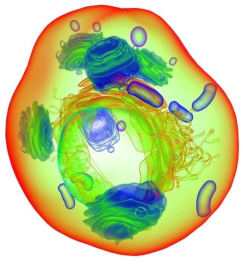
\includegraphics[width=.5\linewidth]{figures/1_cell/cell_1}}%
		\only<2>{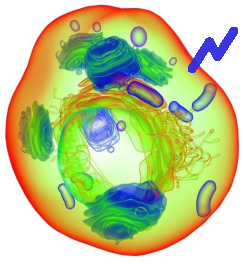
\includegraphics[width=.5\linewidth]{figures/1_cell/cell_2}}%
		\only<3>{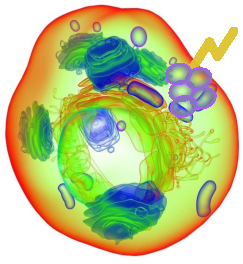
\includegraphics[width=.5\linewidth]{figures/1_cell/cell_3}}%
	\end{center}
	\pnote{Het begint bij de cel, die ook wel de basiseenheid van het leven worden genoemd. Cellen bevatten allerlei moleculen die zij nodig hebben om te kunnen reageren op alle soorten veranderingen in hun omgeving. Als een cel een signaal ontvangt, bijvoorbeeld wanneer een naburige cell iets probeert te zeggen, dan kan de cel daar op reageren door bijvoorbeeld nieuwe eiwitten van een bepaald type aan te maken.}
\end{frame}

\begin{frame}
	\frametitle{Hoe maken cellen eiwitten aan?}
	\begin{center}
		\only<1>{
\includegraphics[width=\linewidth]{figures/2_centraldogma/central_dogma_1.pdf}}%
		\only<2>{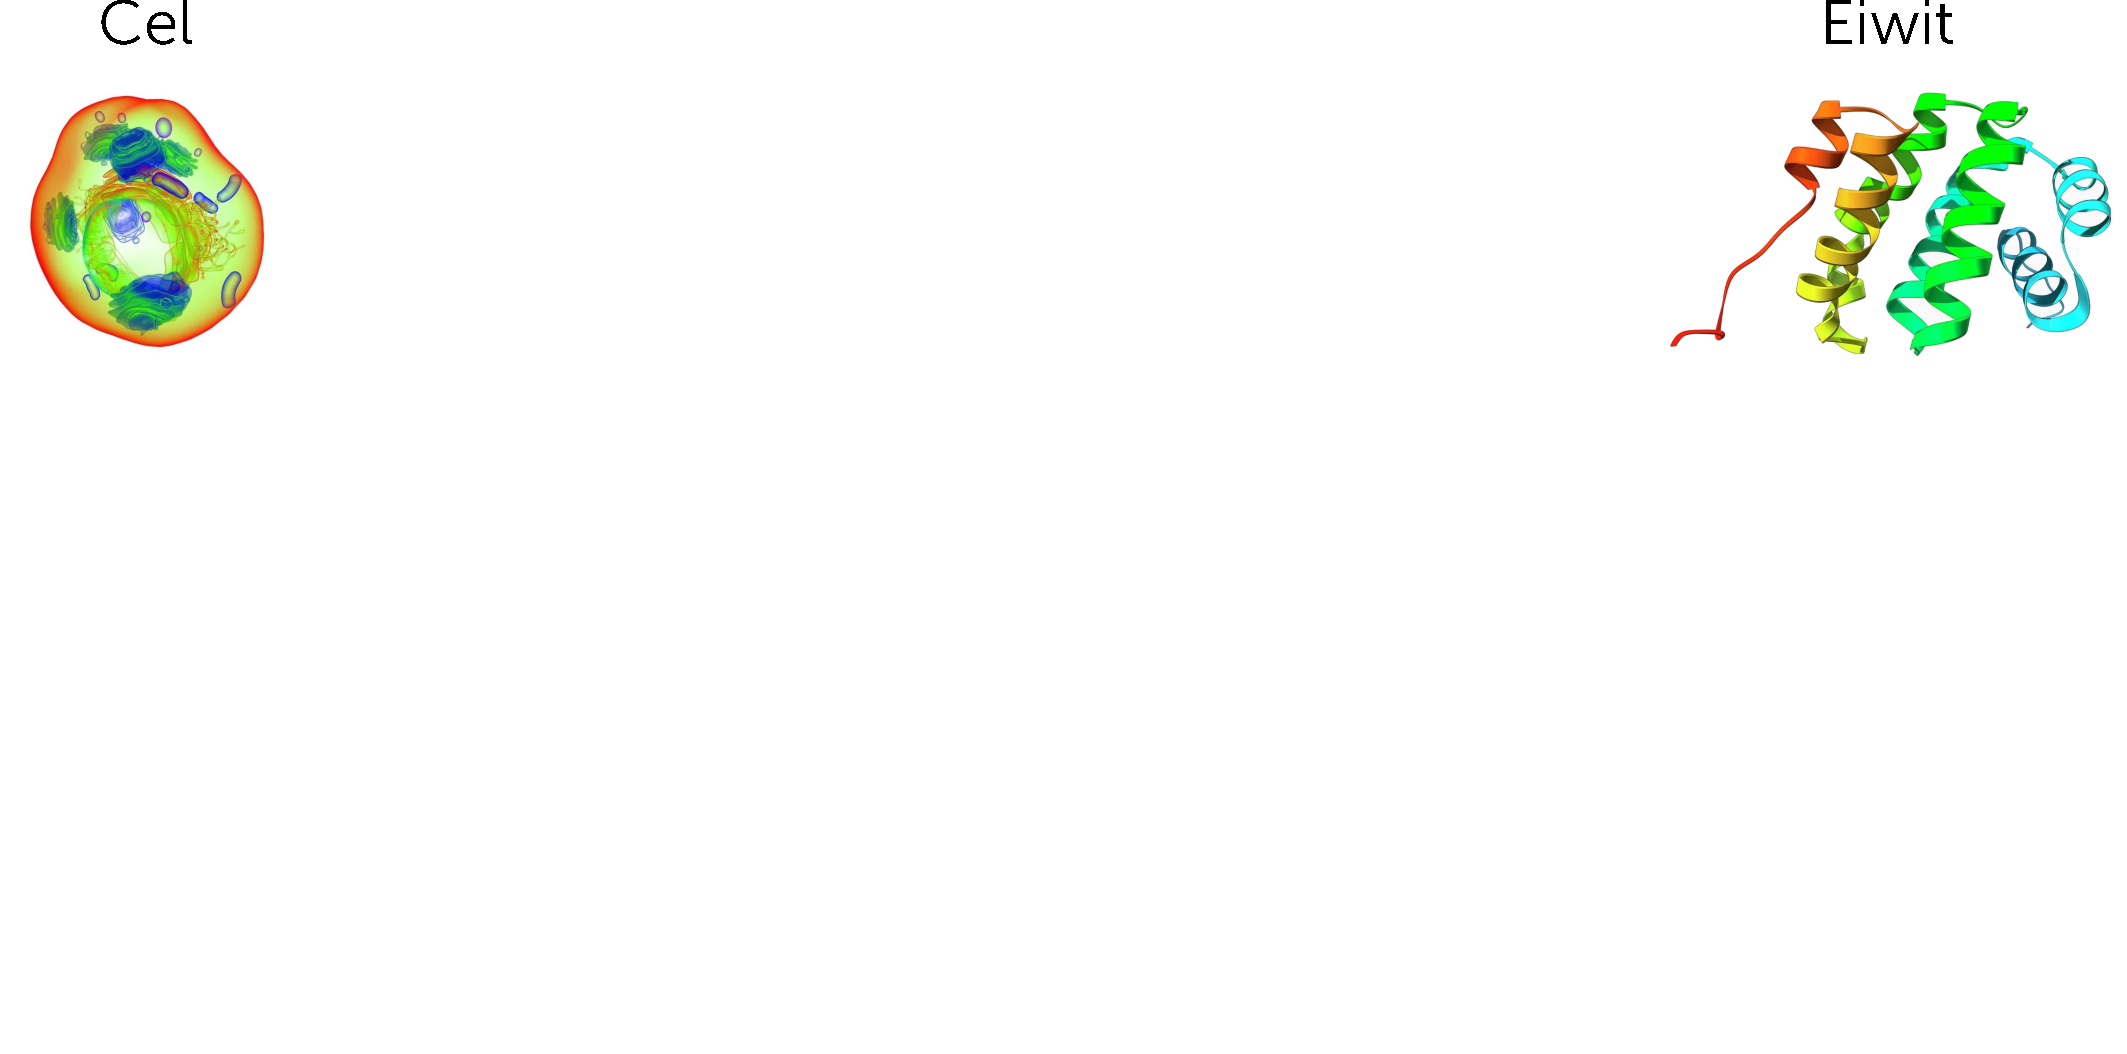
\includegraphics[width=\linewidth]{figures/2_centraldogma/central_dogma_2.pdf}}%
		\only<3>{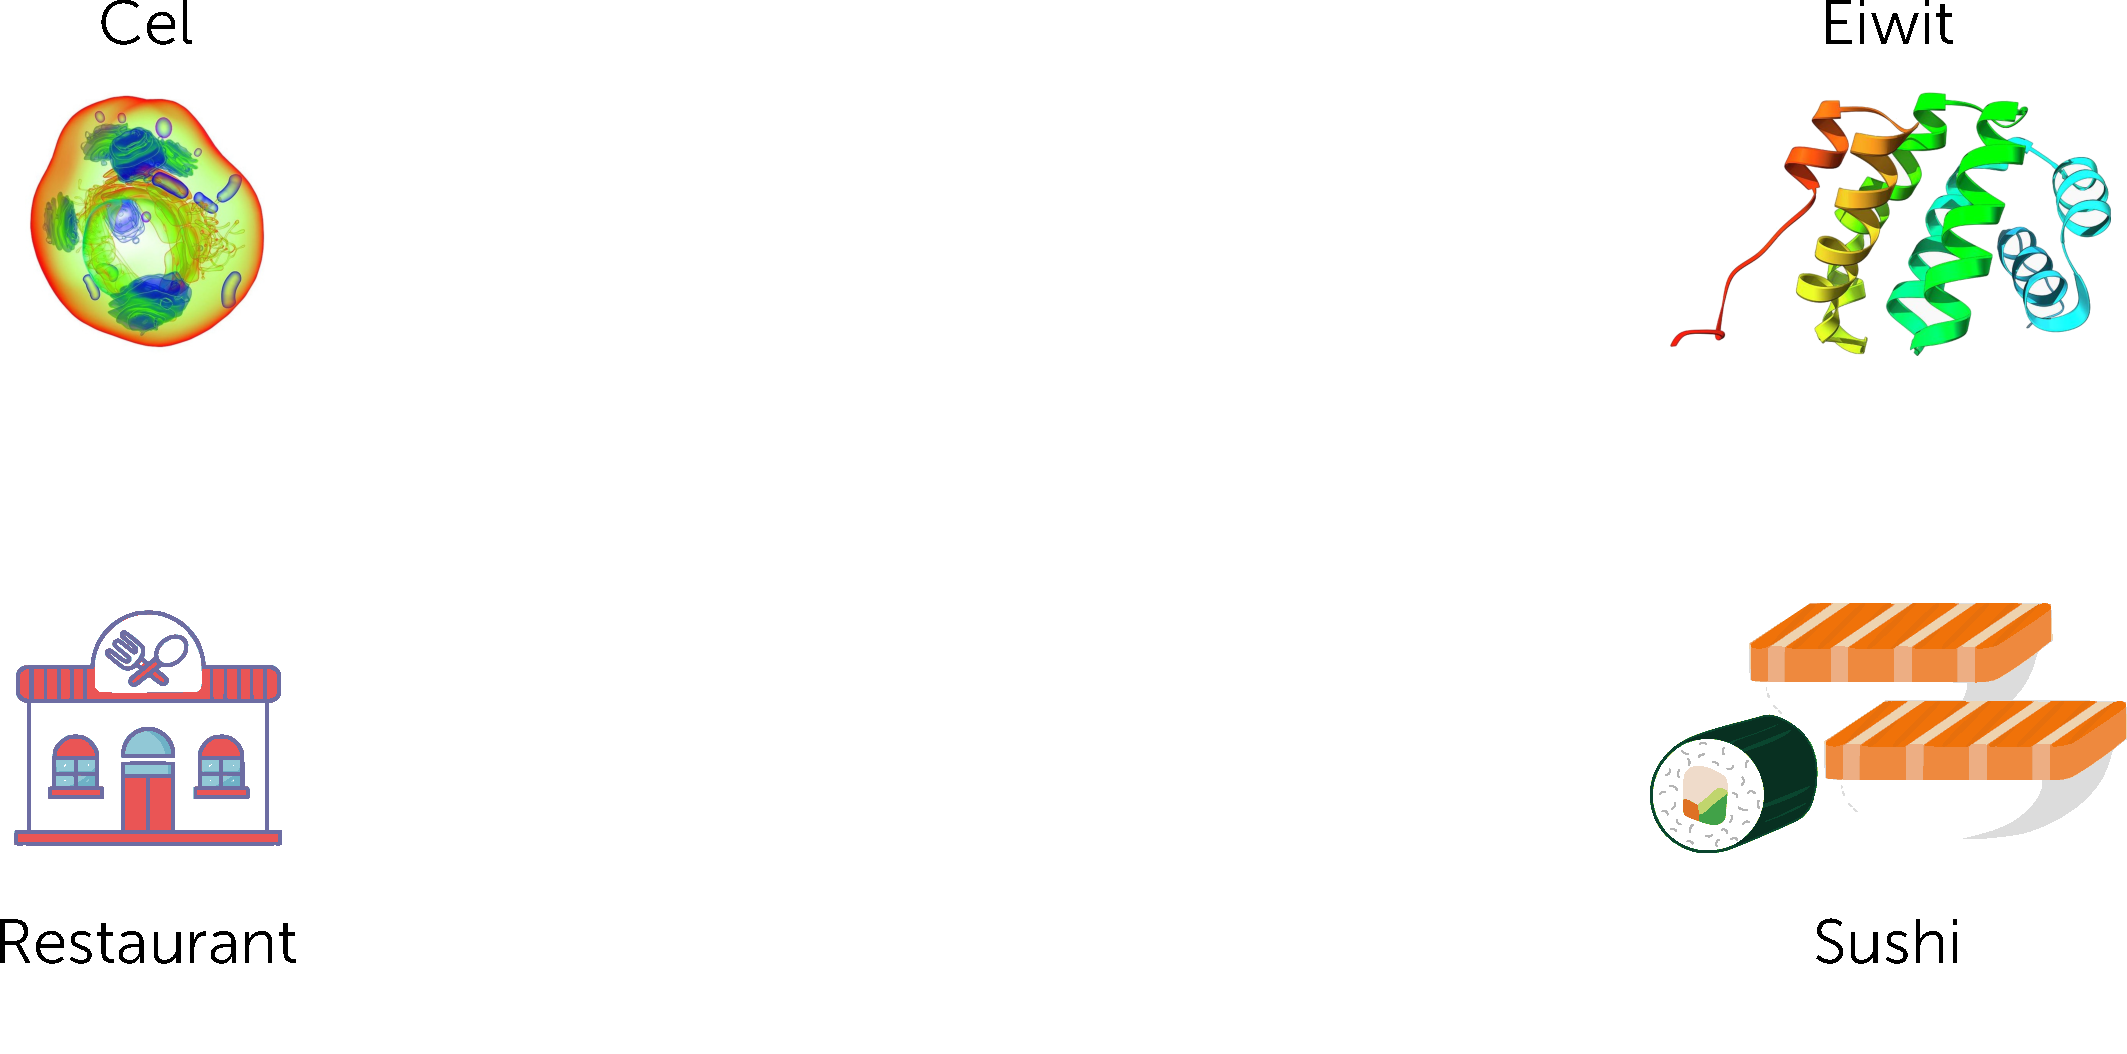
\includegraphics[width=\linewidth]{figures/2_centraldogma/central_dogma_3.pdf}}%
		\only<4>{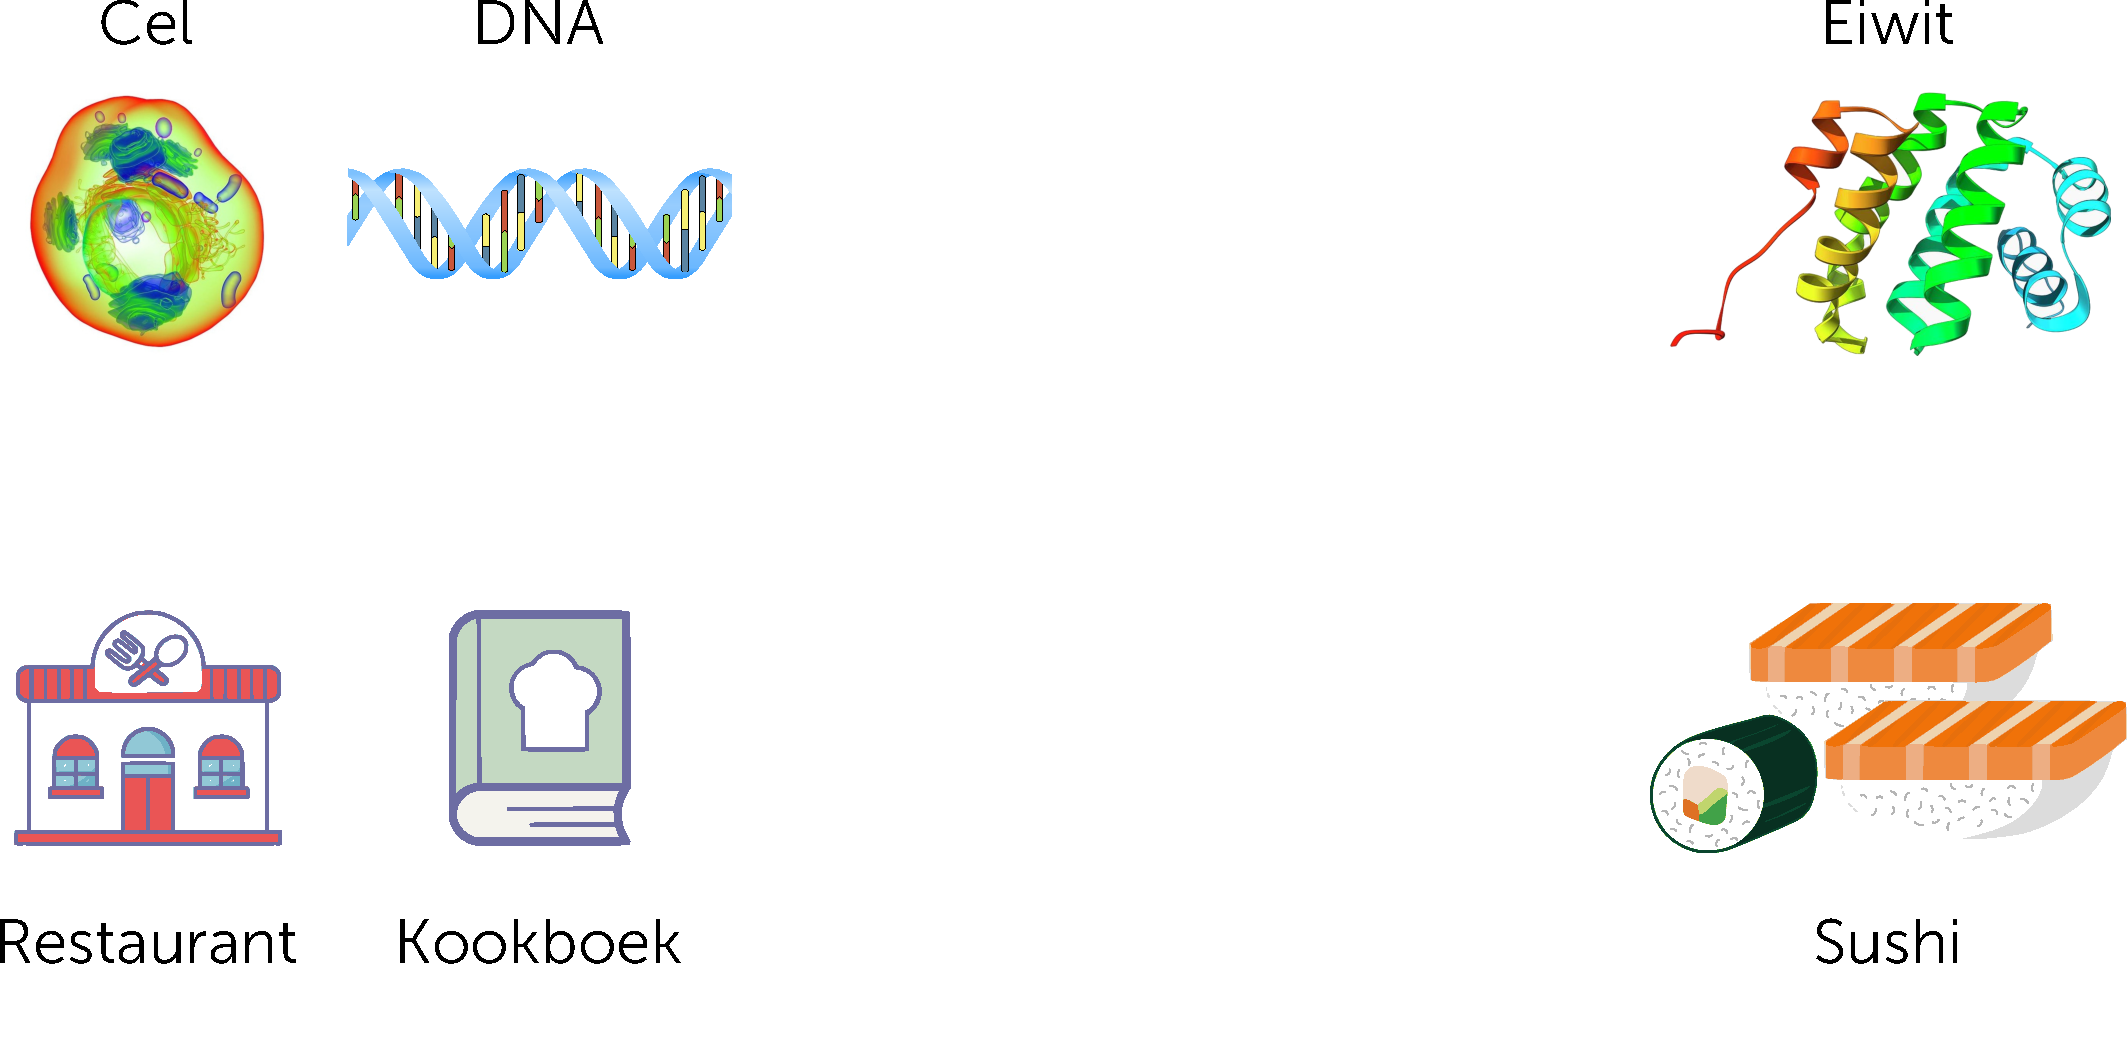
\includegraphics[width=\linewidth]{figures/2_centraldogma/central_dogma_4.pdf}}%
		\only<5>{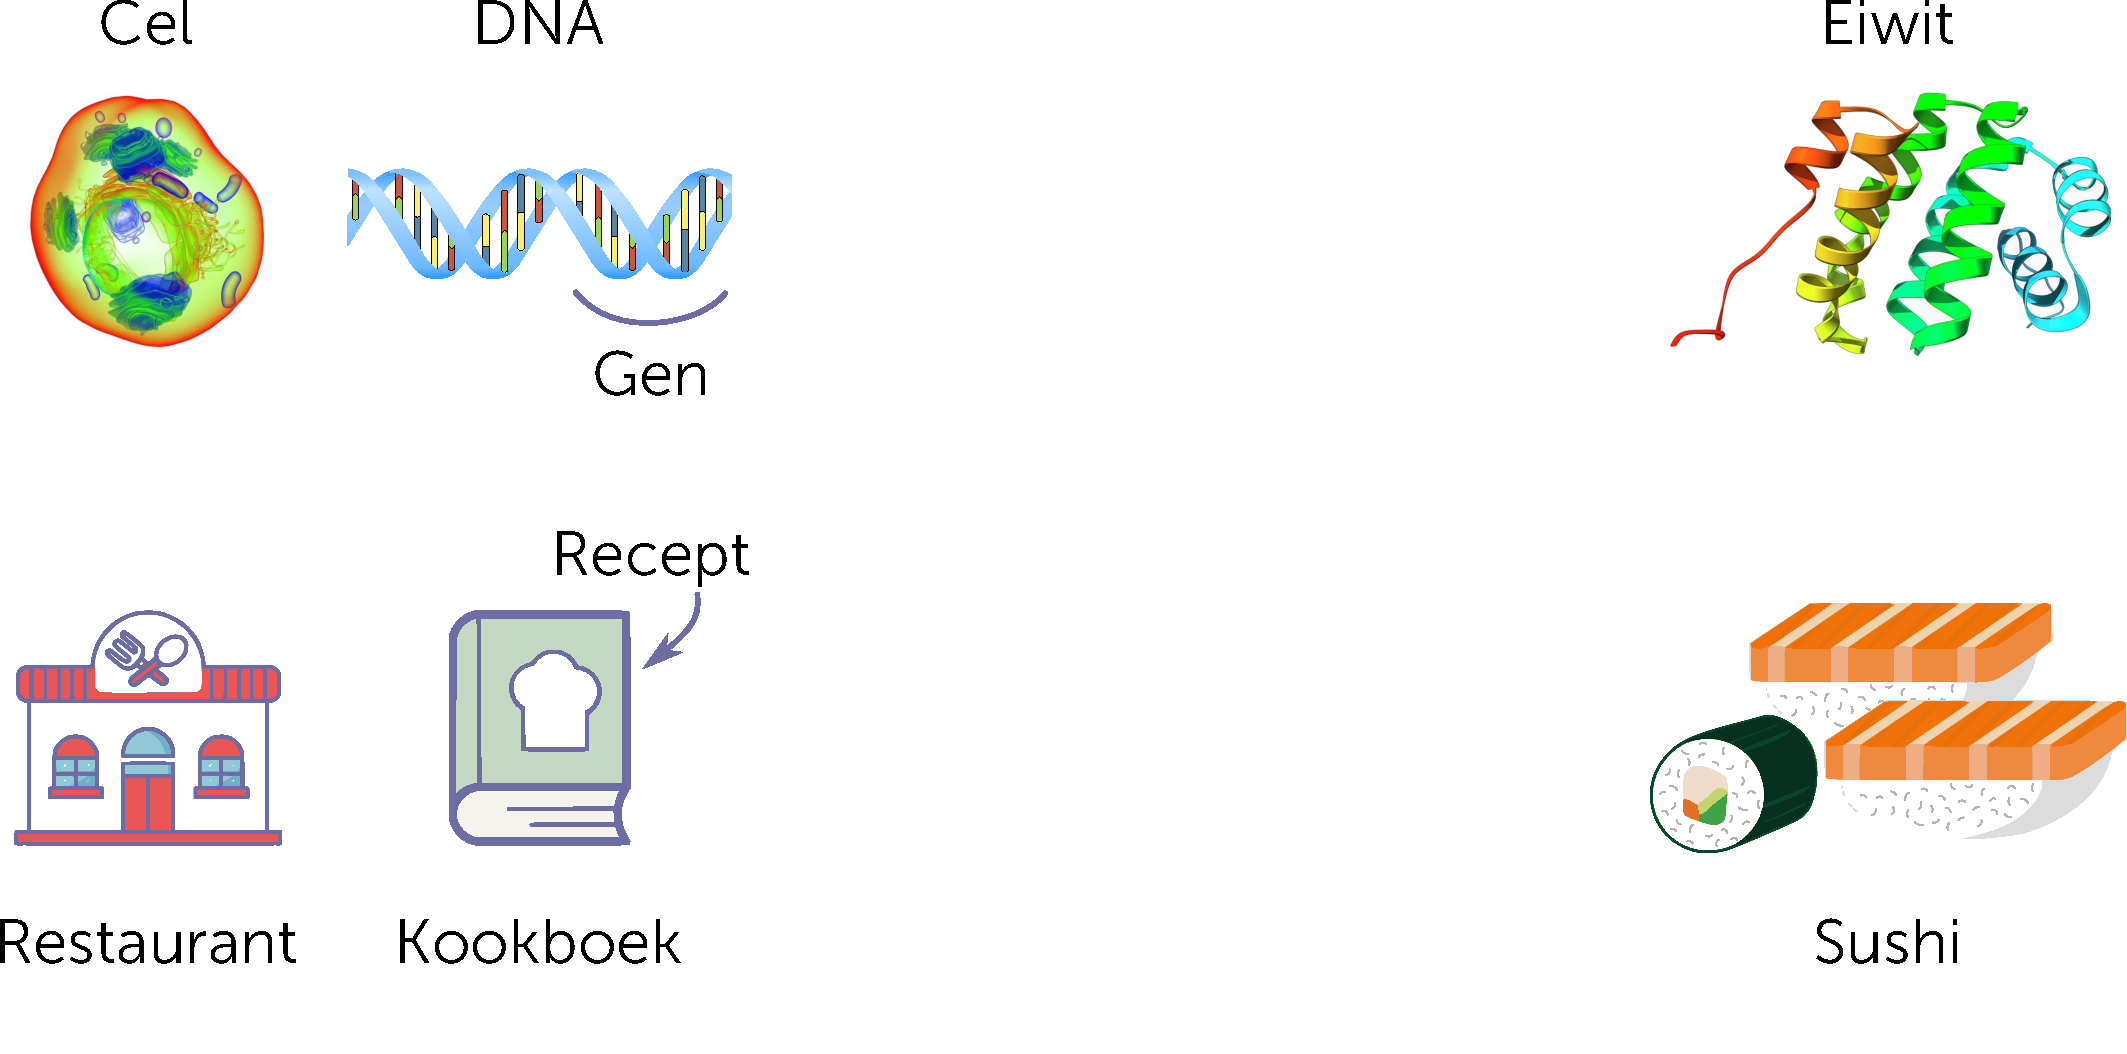
\includegraphics[width=\linewidth]{figures/2_centraldogma/central_dogma_5.pdf}}%
		\only<6>{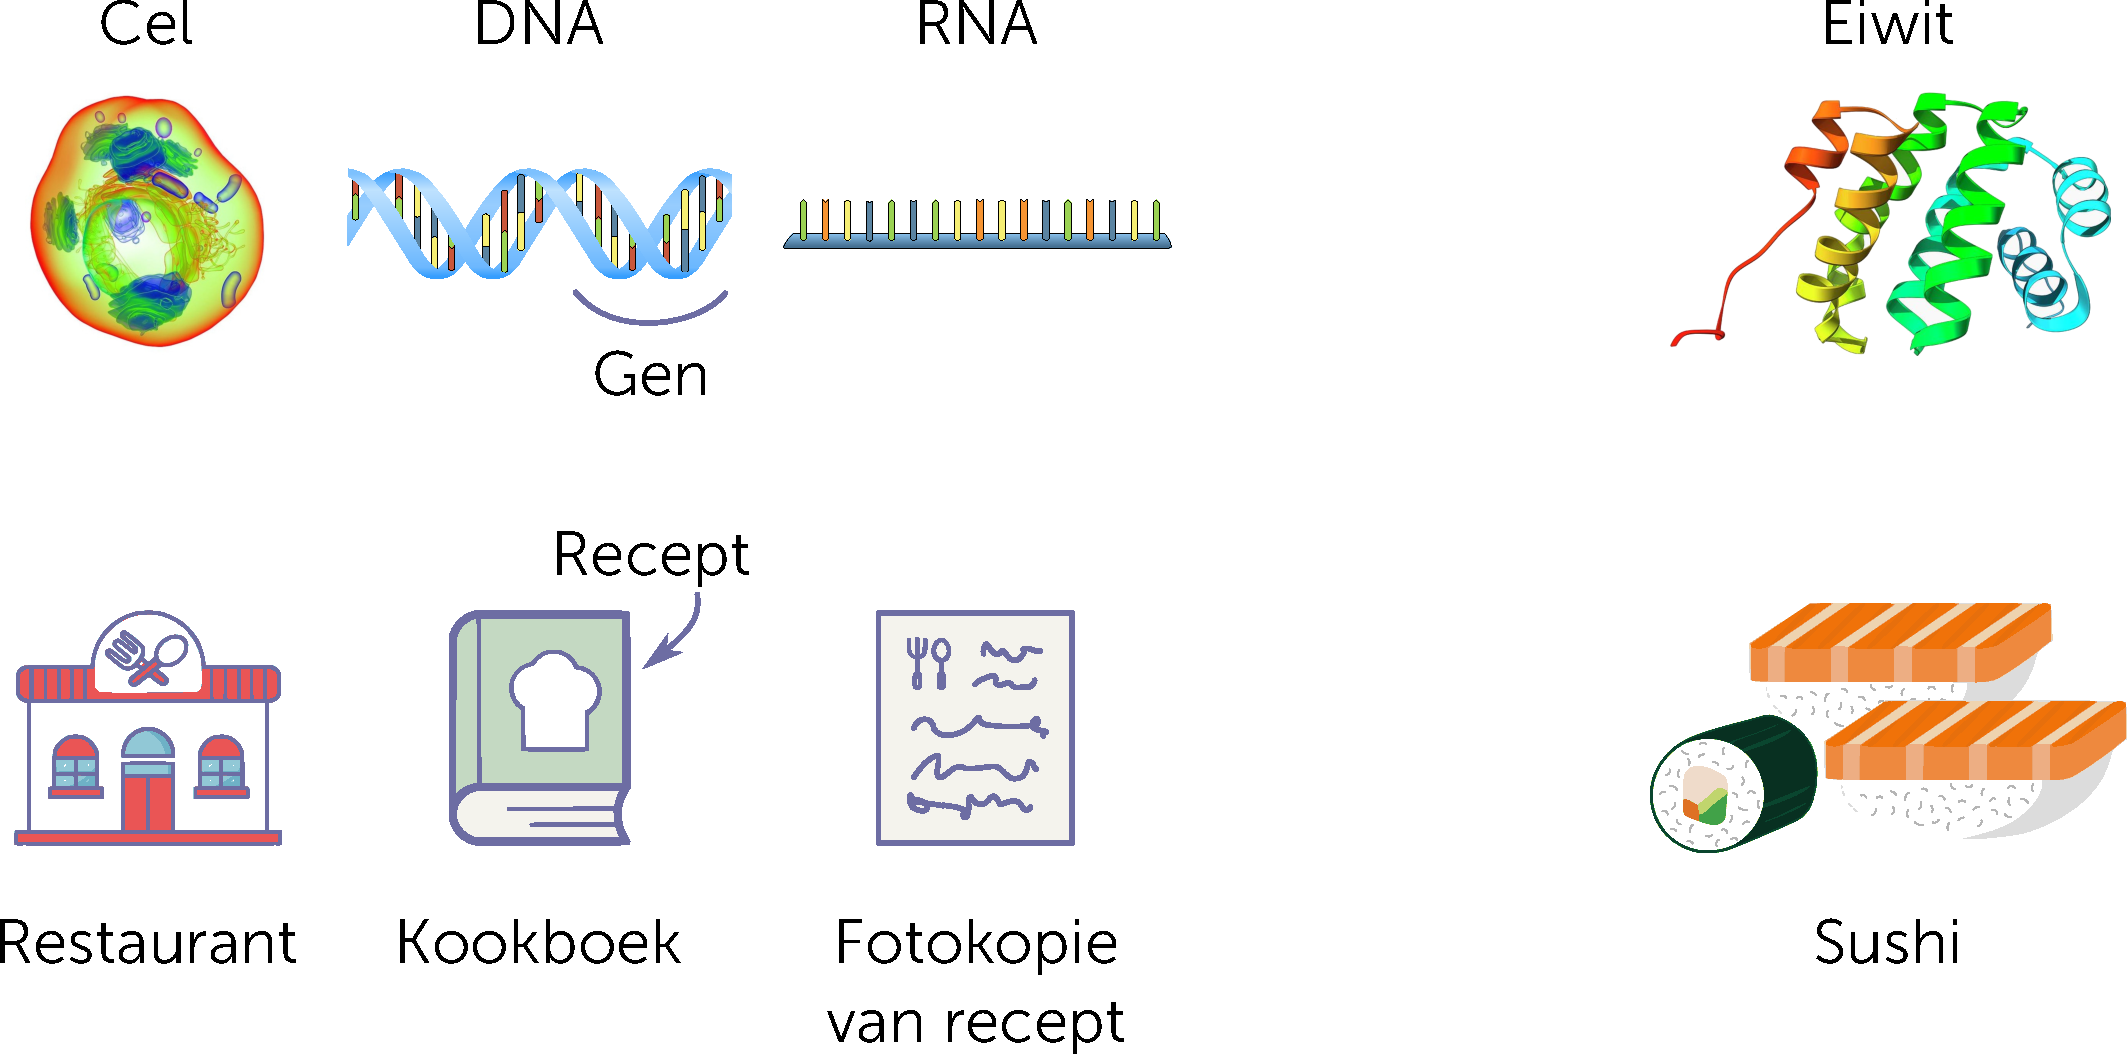
\includegraphics[width=\linewidth]{figures/2_centraldogma/central_dogma_6.pdf}}%
		\only<6>{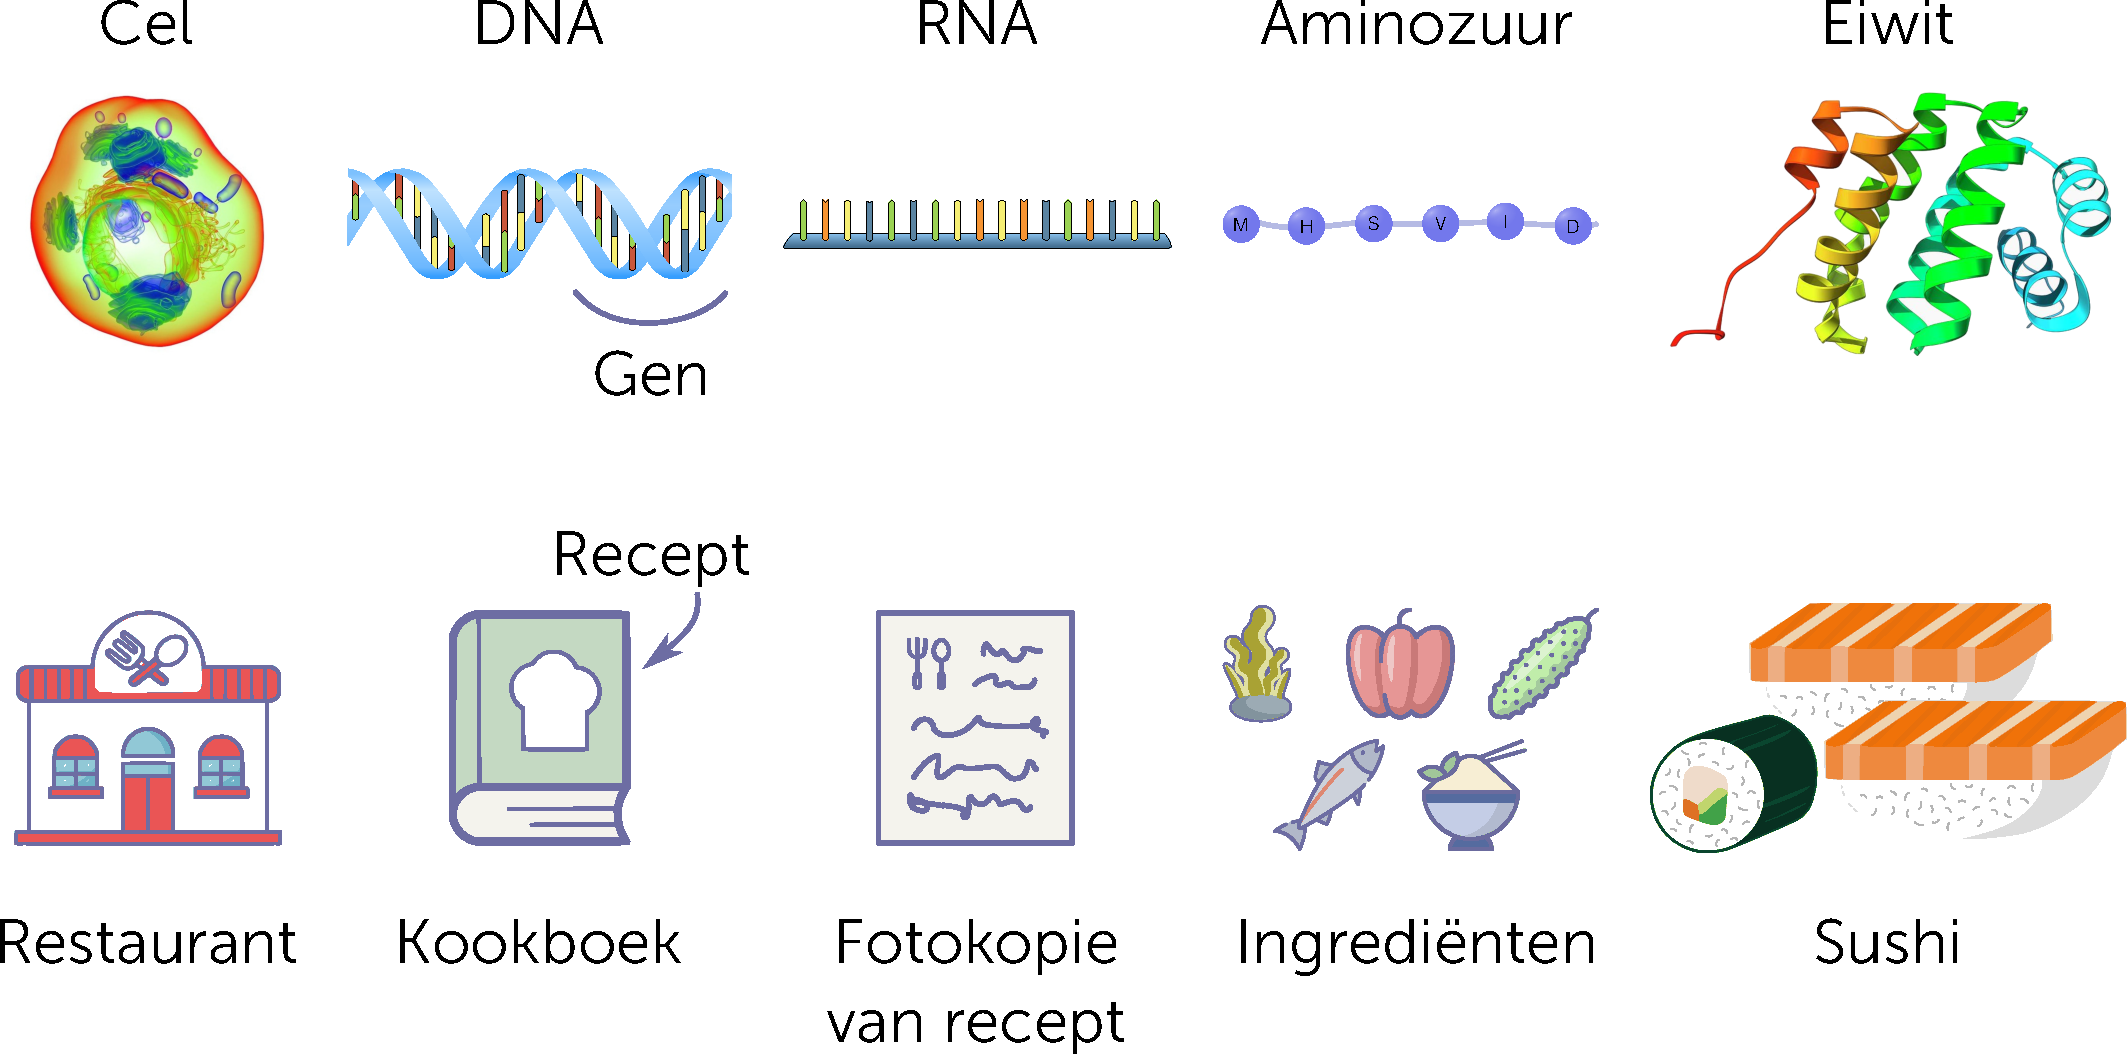
\includegraphics[width=\linewidth]{figures/2_centraldogma/central_dogma_7.pdf}}%
	\end{center}

\end{frame}

\begin{frame}
	\frametitle{Het menselijk lichaam bevat >210 soorten cellen}
	\begin{center}
		\only<1>{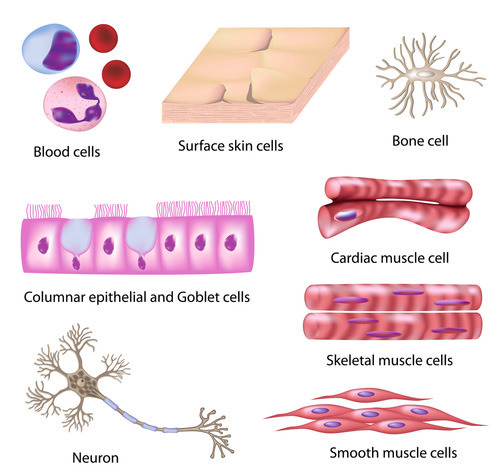
\includegraphics[width=.6\linewidth]{figures/3_celtypes/celtypes.jpg}}%
	\end{center}
	\uncover<1>{(placeholder figuur)}

\end{frame}

\begin{frame}
	\frametitle{Cellen kunnen ontwikkelen van één type naar een ander}
	\begin{center}
		\only<1->{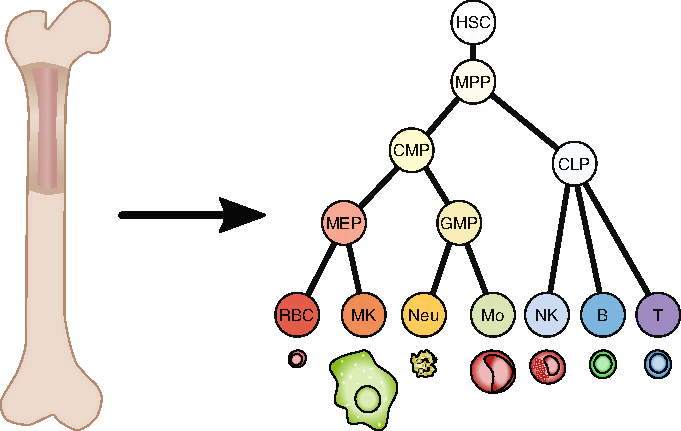
\includegraphics[width=.8\linewidth]{figures/3_celtypes/lineagetree.pdf}}%
	\end{center}

\end{frame}

\begin{frame}
	\frametitle{Welke types cellen komen voor in een populatie?}
	\begin{center}
		\only<1>{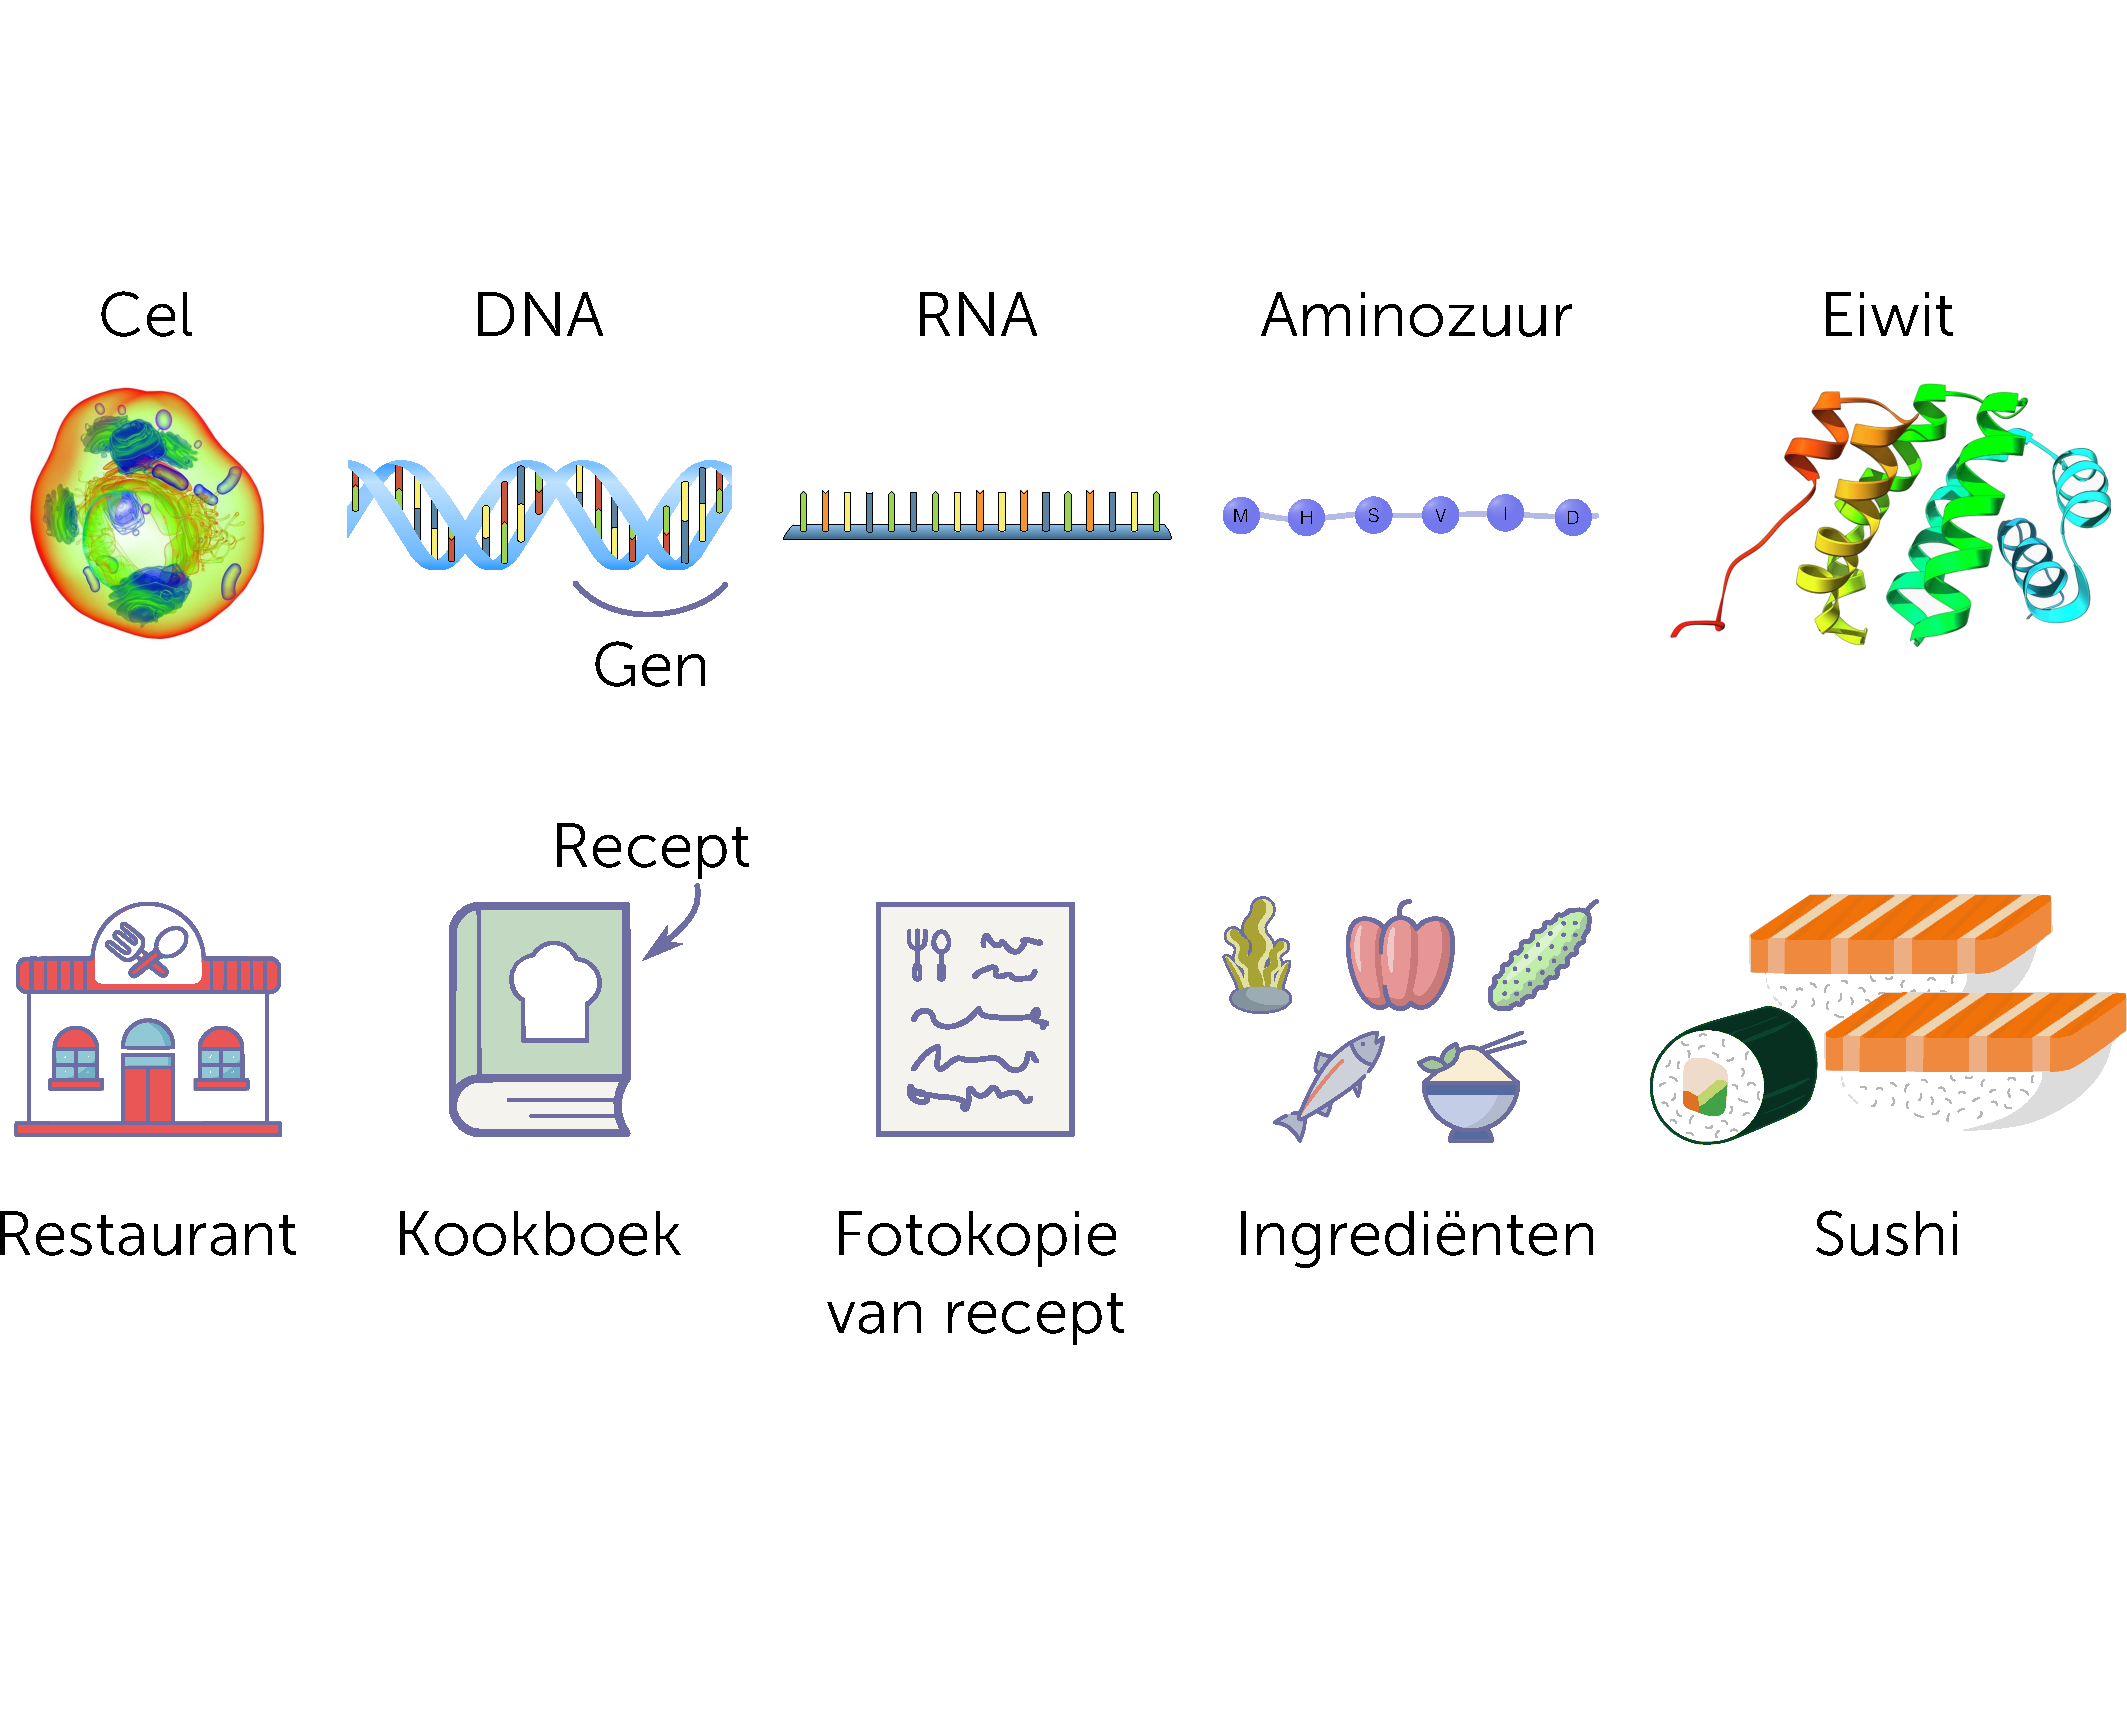
\includegraphics[width=.9\linewidth]{figures/4_singlecellomics/scomics_1.pdf}}%
		\only<2>{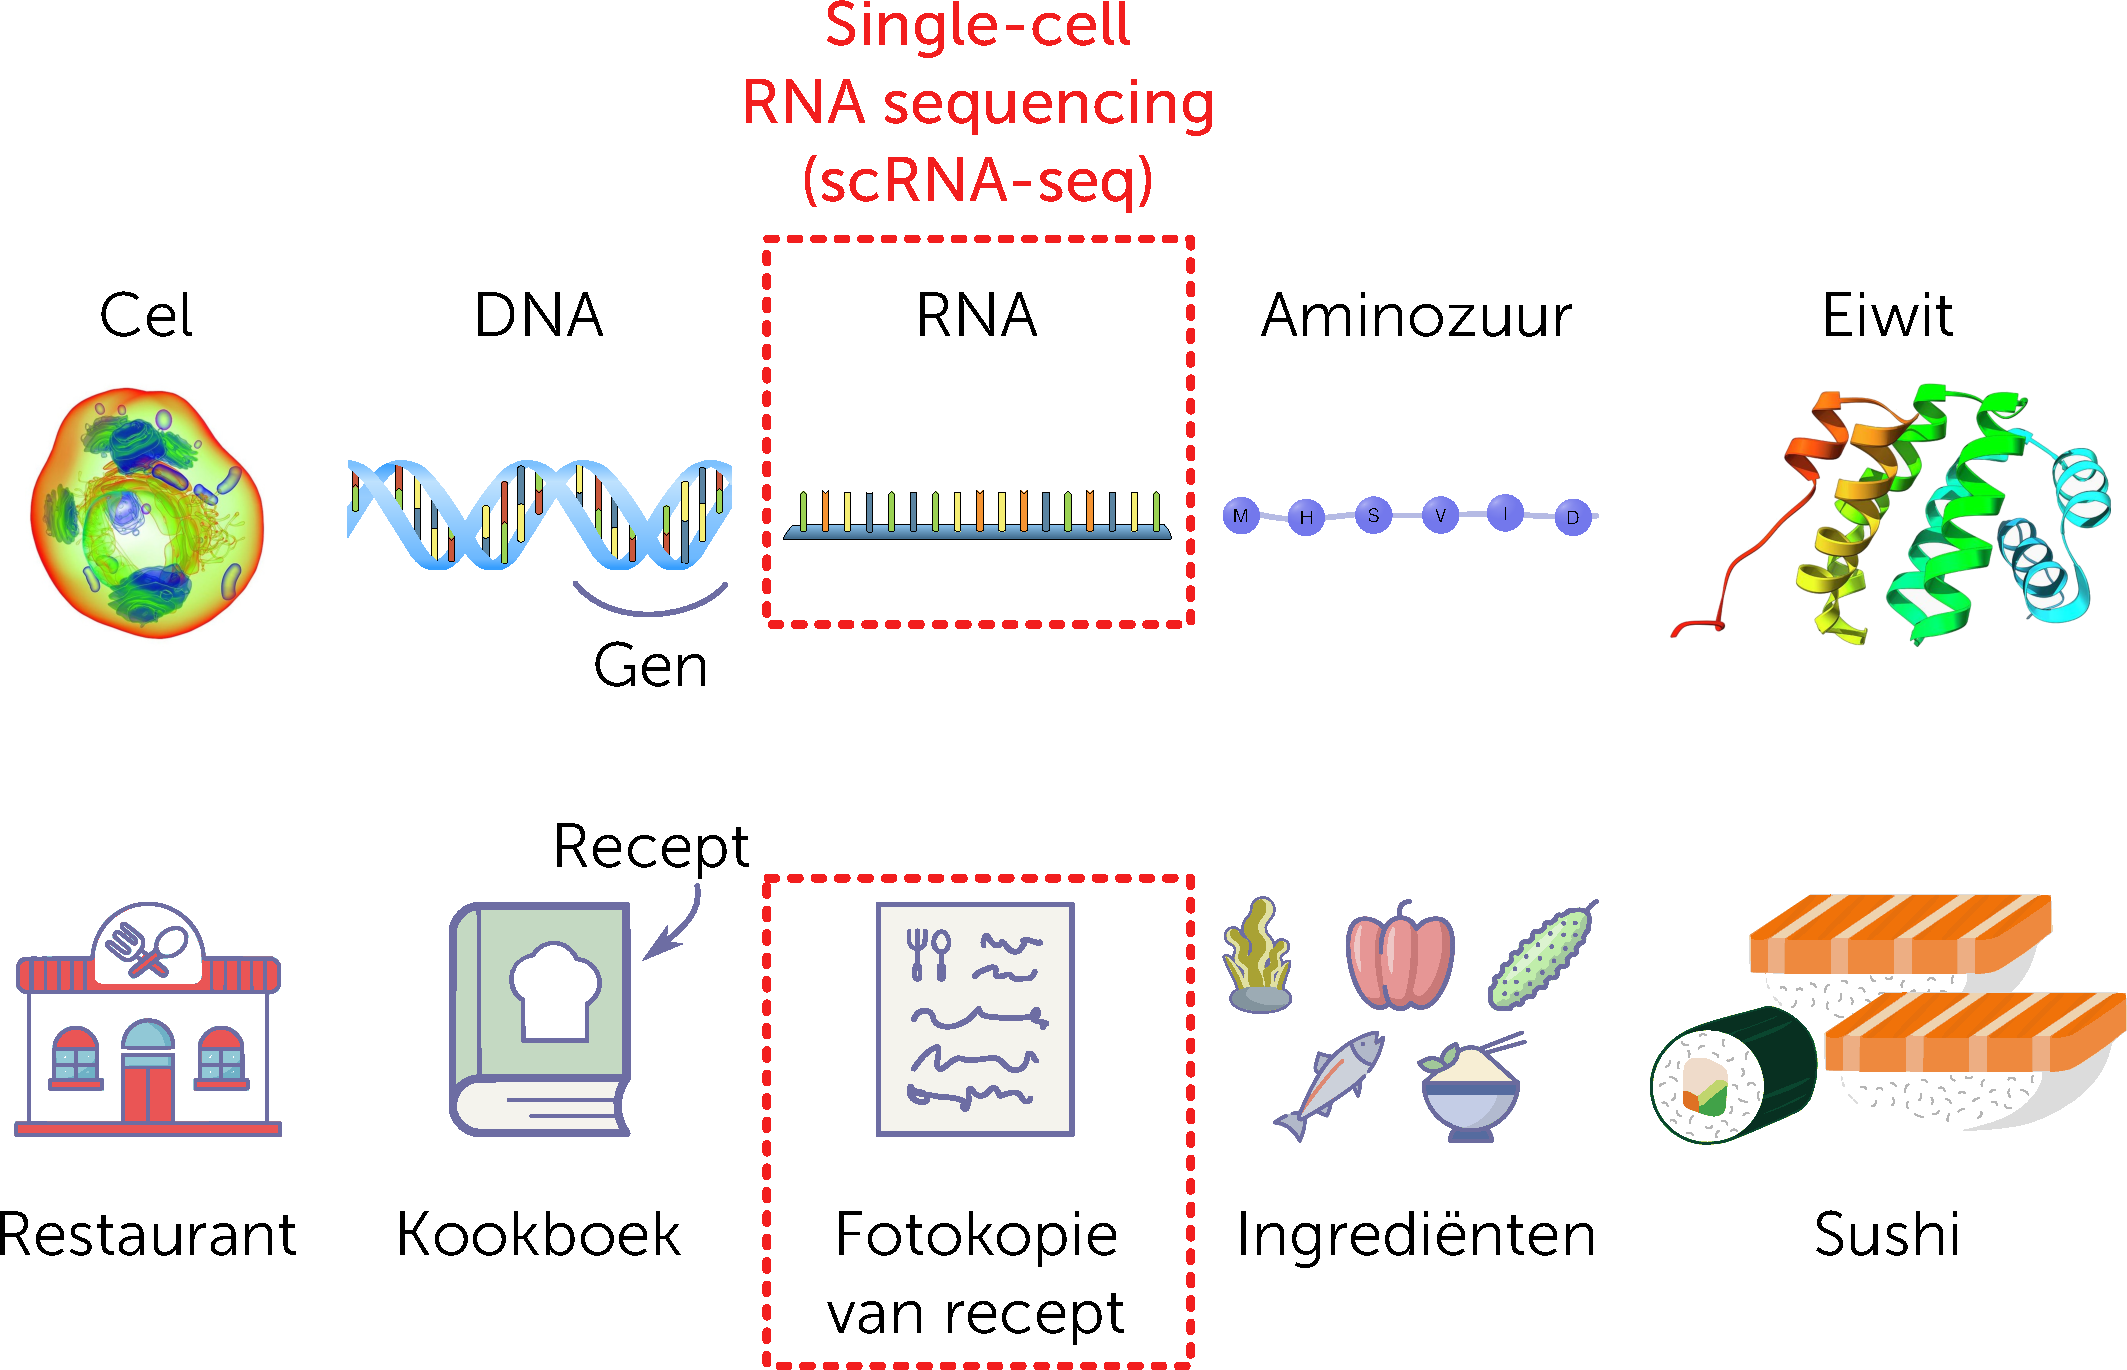
\includegraphics[width=.9\linewidth]{figures/4_singlecellomics/scomics_2.pdf}}%
		\only<3>{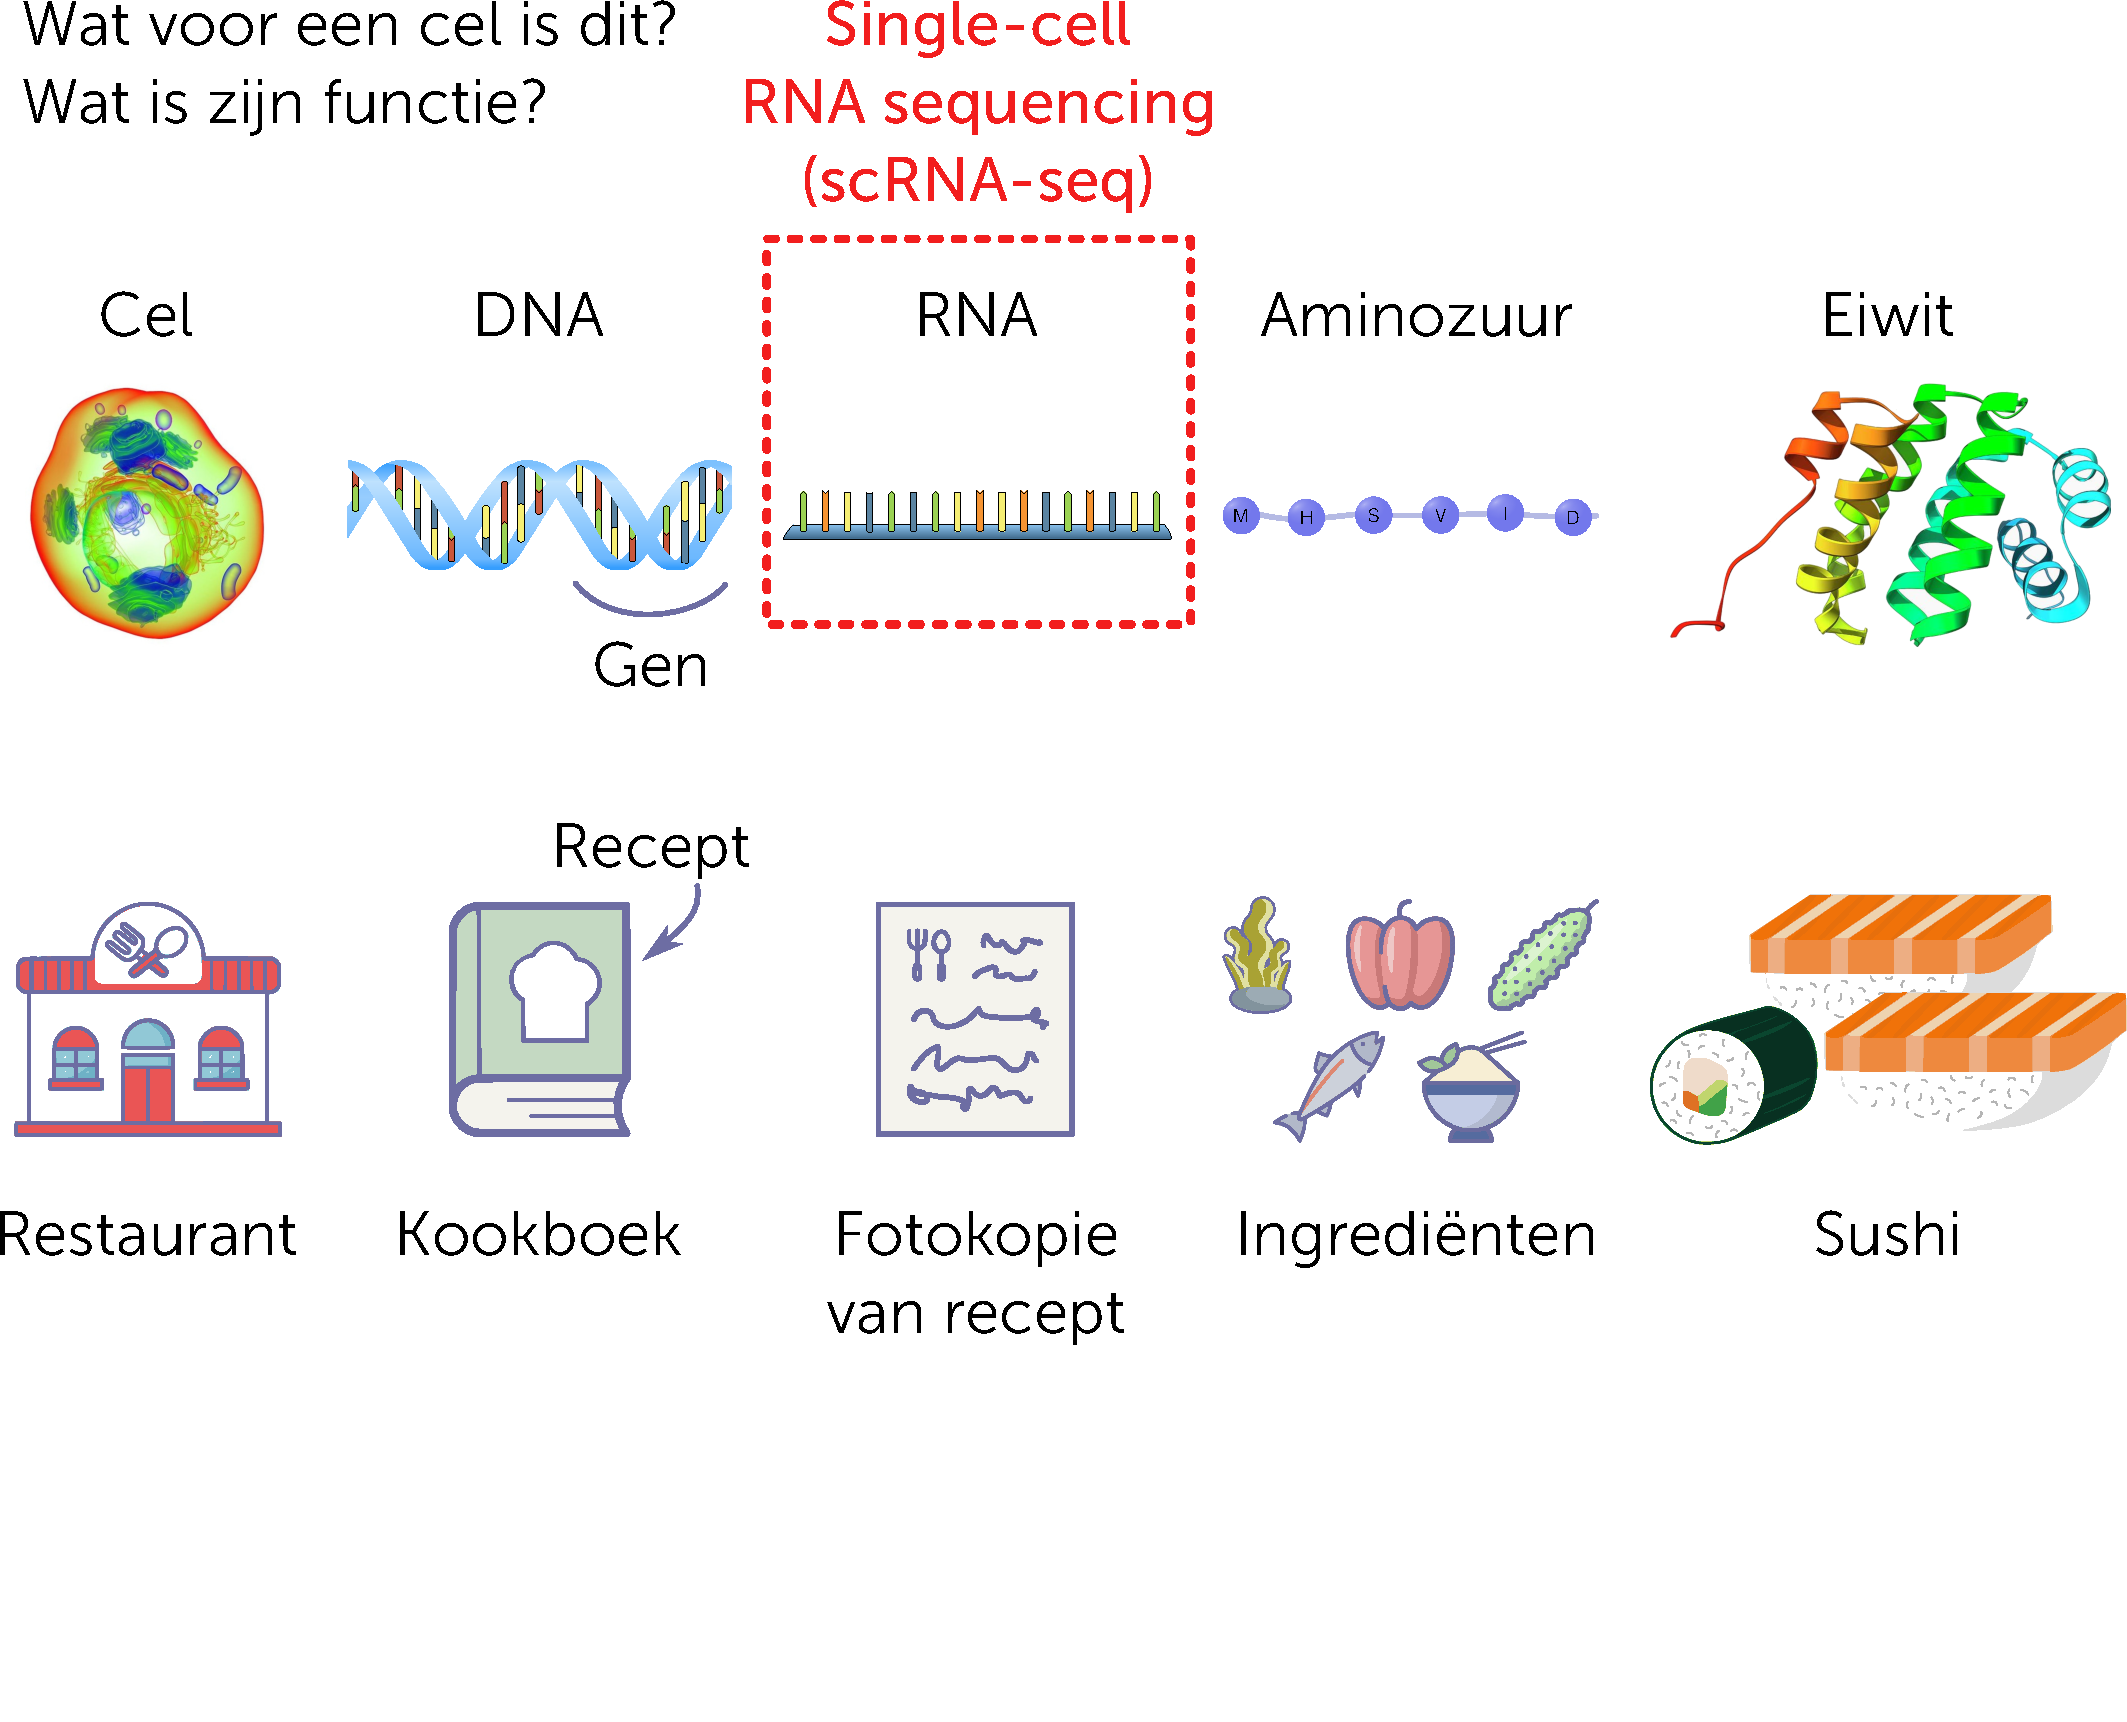
\includegraphics[width=.9\linewidth]{figures/4_singlecellomics/scomics_3.pdf}}%
		\only<4>{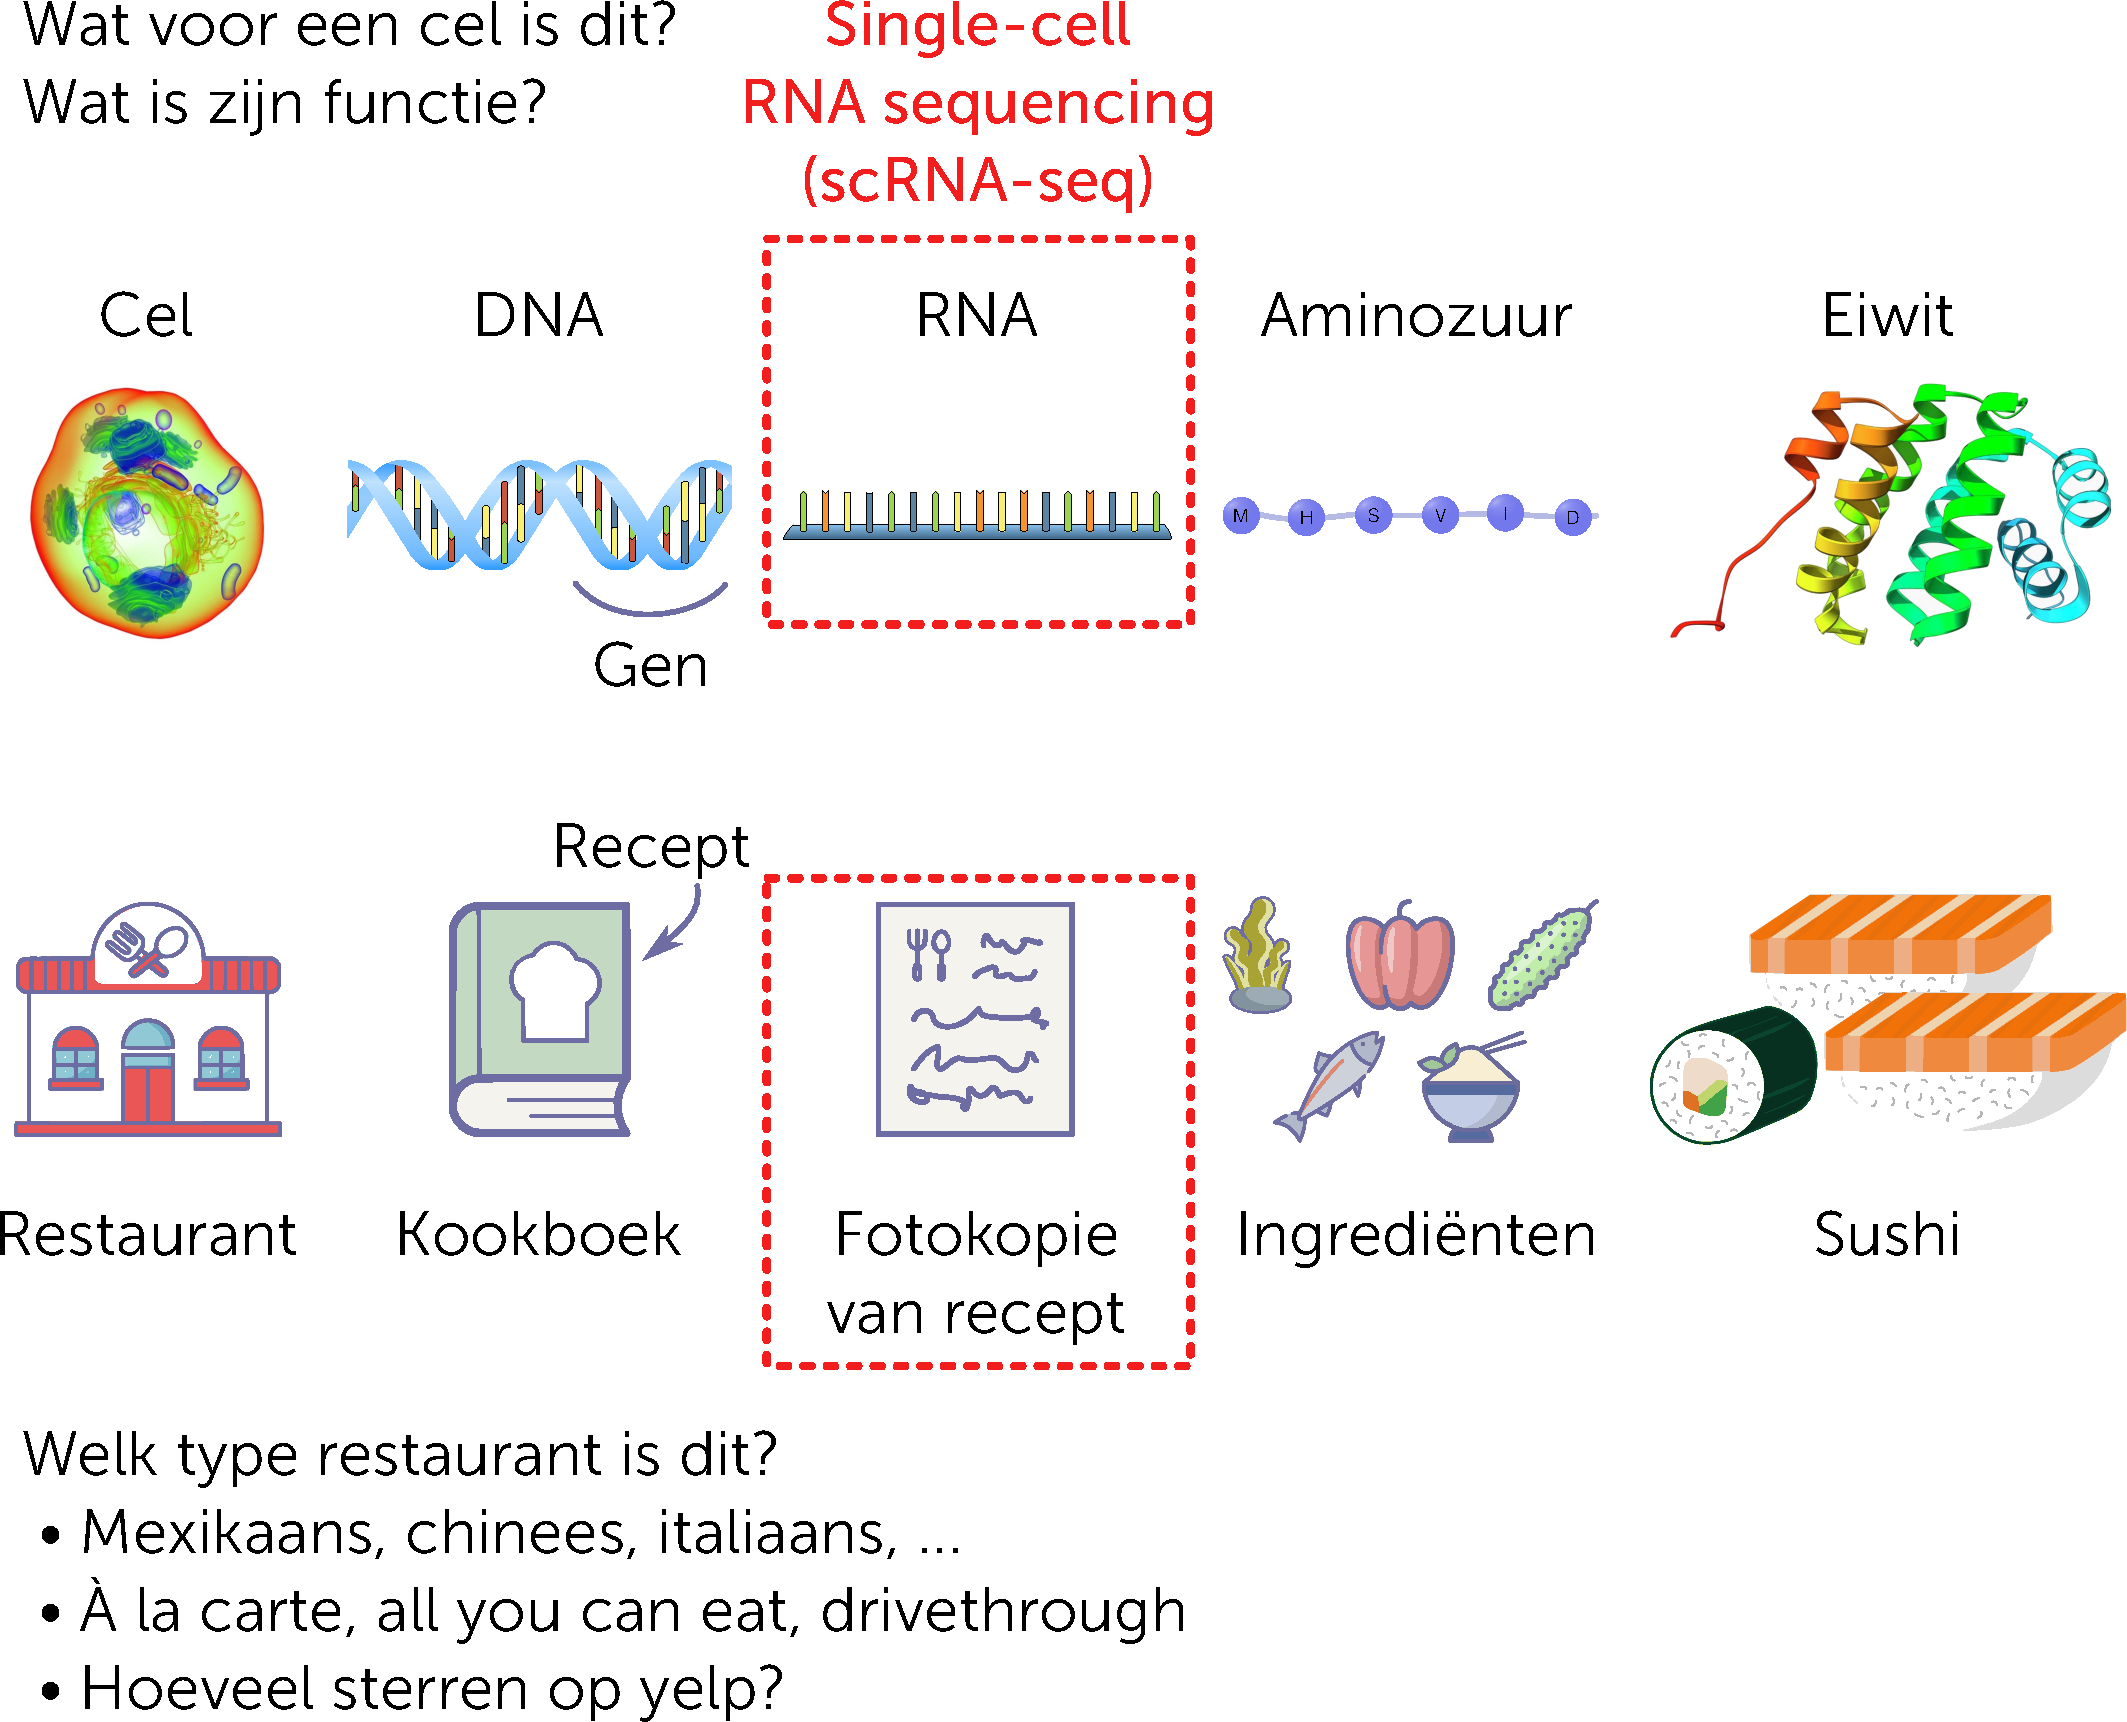
\includegraphics[width=.9\linewidth]{figures/4_singlecellomics/scomics_4.pdf}}%
	\end{center}

\end{frame}
	

\begin{frame}
	\frametitle{2014: doorbraak in schaalbaarheid van scRNA-seq}
	\begin{center}
		\only<1>{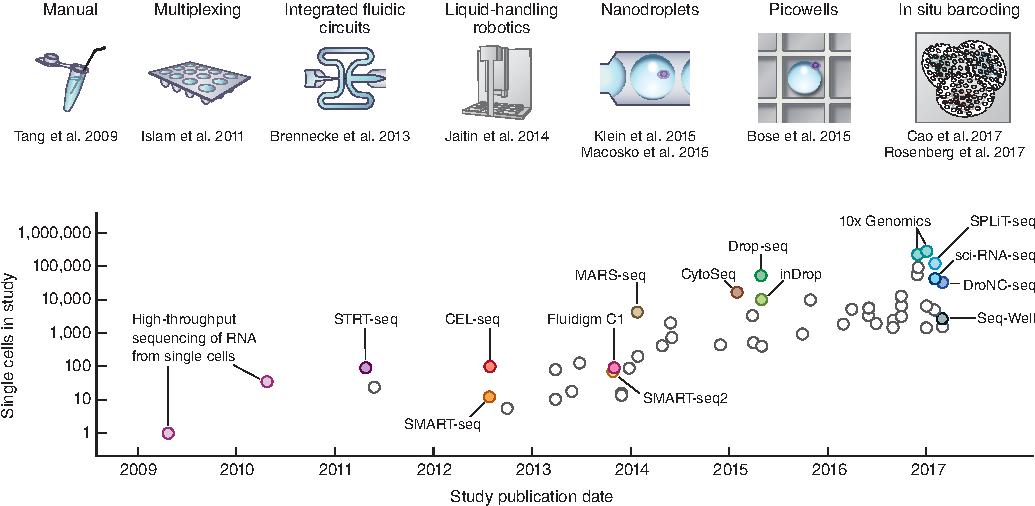
\includegraphics[width=\linewidth]{figures/4_singlecellomics/scaling.pdf}}%
	\end{center}
\end{frame}
	
\begin{frame}
	\frametitle{Voorbeeld van een scRNA-seq technologie: Drop-seq}
  \begin{center}
		\movie{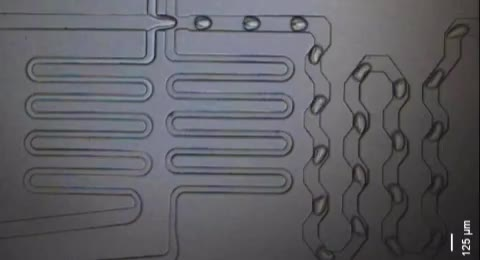
\includegraphics[width=\textwidth]{figures/4_singlecellomics/DropSeq_thumbnail.jpg}}{figures/4_singlecellomics/DropSeq.avi}%
	\end{center}
\end{frame}


\begin{frame}
	\frametitle{Moleculen tellen met scRNA-seq}
	\begin{center}
		\only<1>{
\includegraphics[width=.8\linewidth]{figures/4_singlecellomics/rnaseq_1.pdf}}%
		\only<2>{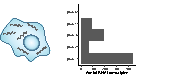
\includegraphics[width=.8\linewidth]{figures/4_singlecellomics/rnaseq_2.pdf}}%
		\only<3>{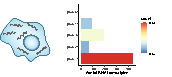
\includegraphics[width=.8\linewidth]{figures/4_singlecellomics/rnaseq_3.pdf}}%
		\only<4>{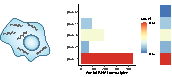
\includegraphics[width=.8\linewidth]{figures/4_singlecellomics/rnaseq_4.pdf}}%
		\only<5>{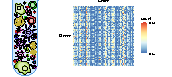
\includegraphics[width=\linewidth]{figures/4_singlecellomics/rnaseq_5.pdf}}%
	\end{center}

\end{frame}

\begin{frame}
	\frametitle{Cellen ordenen met SCORPIUS}
	\begin{center}
		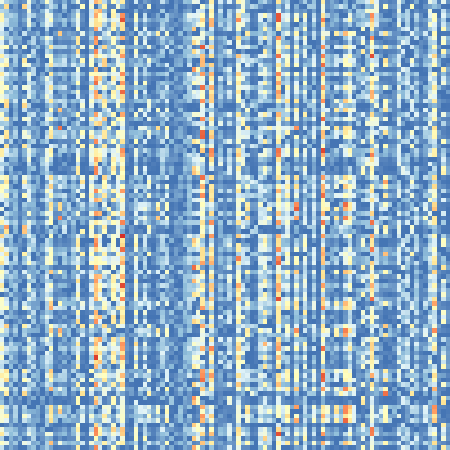
\includegraphics[width=.35\linewidth]{figures/4_singlecellomics/rnaseq_plot.pdf}%
		\uncover<2->{%
			\only<1-2>{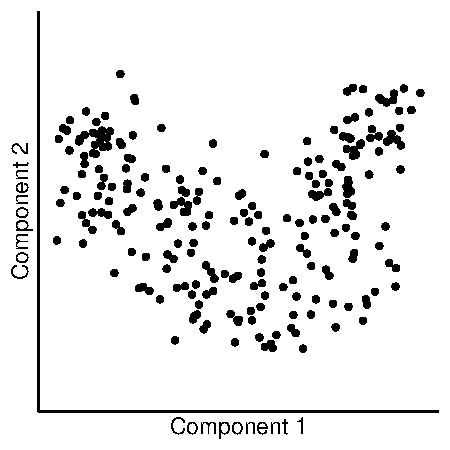
\includegraphics[width=.35\linewidth]{figures/5_scorpius/dimred.pdf}}%
			\only<3->{\movie{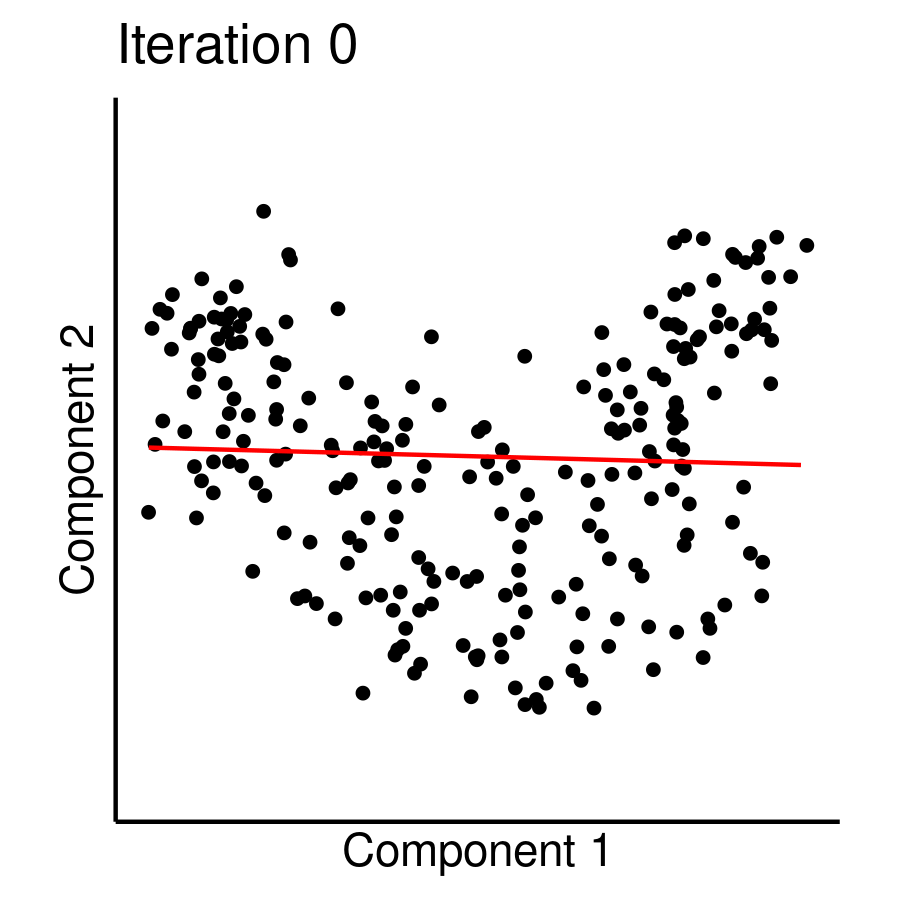
\includegraphics[width=.35\linewidth]{figures/5_scorpius/princurve_it0.png}}{figures/5_scorpius/princurve_loop.avi}}%
			\hspace{.116666\linewidth}
		}\\%
		\uncover<4->{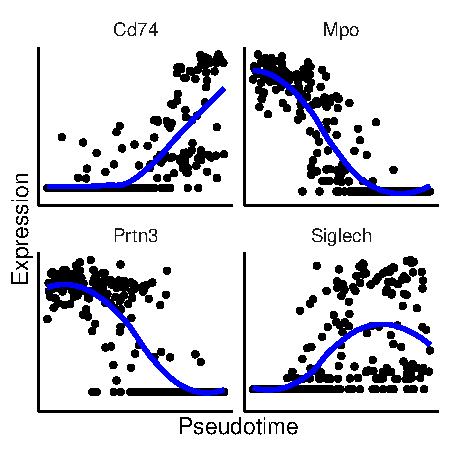
\includegraphics[width=.35\linewidth]{figures/5_scorpius/expr_time.pdf}}%
		\uncover<5->{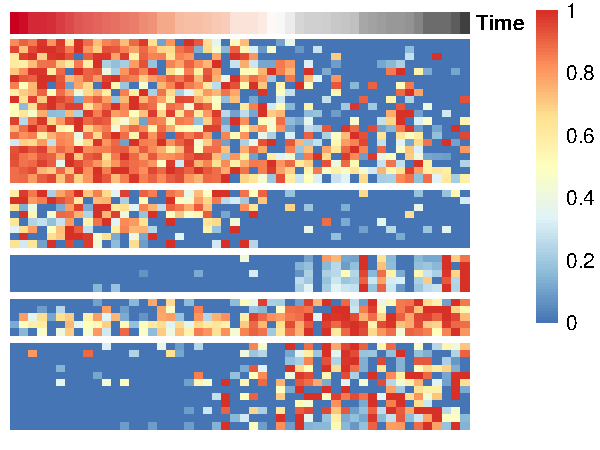
\includegraphics[width=.46666\linewidth]{figures/5_scorpius/heatmap.pdf}}%
	\end{center}
\end{frame}

\begin{frame}
	\frametitle{Niet alle datasets zijn even gemakkelijk}
	\begin{center}
		\only<1>{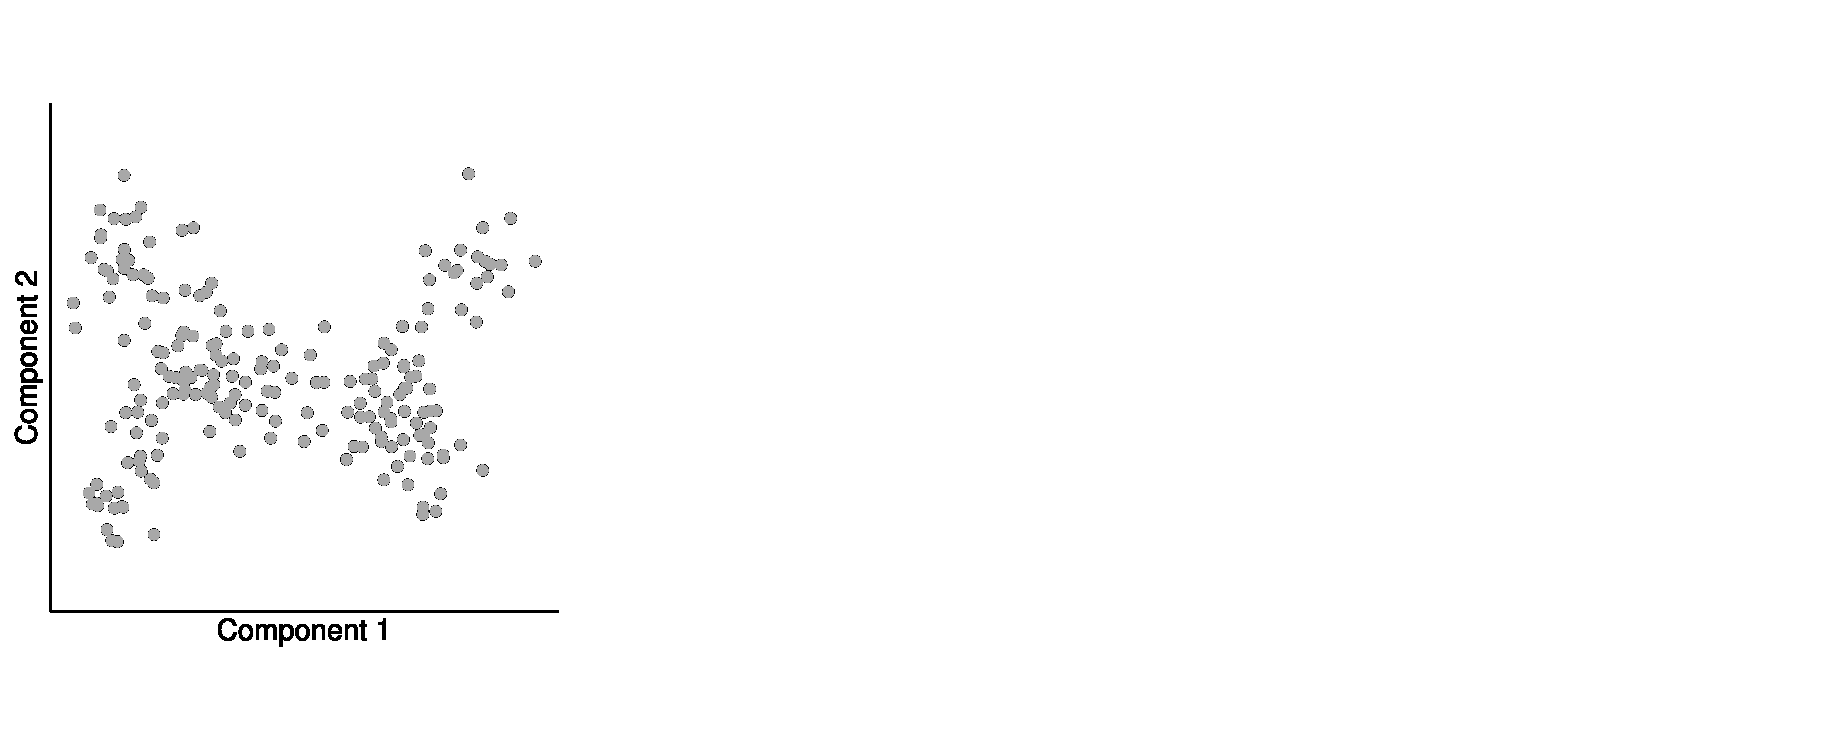
\includegraphics[width=\linewidth]{figures/6_multifurcation/plots_1.pdf}}%
		\only<2-3>{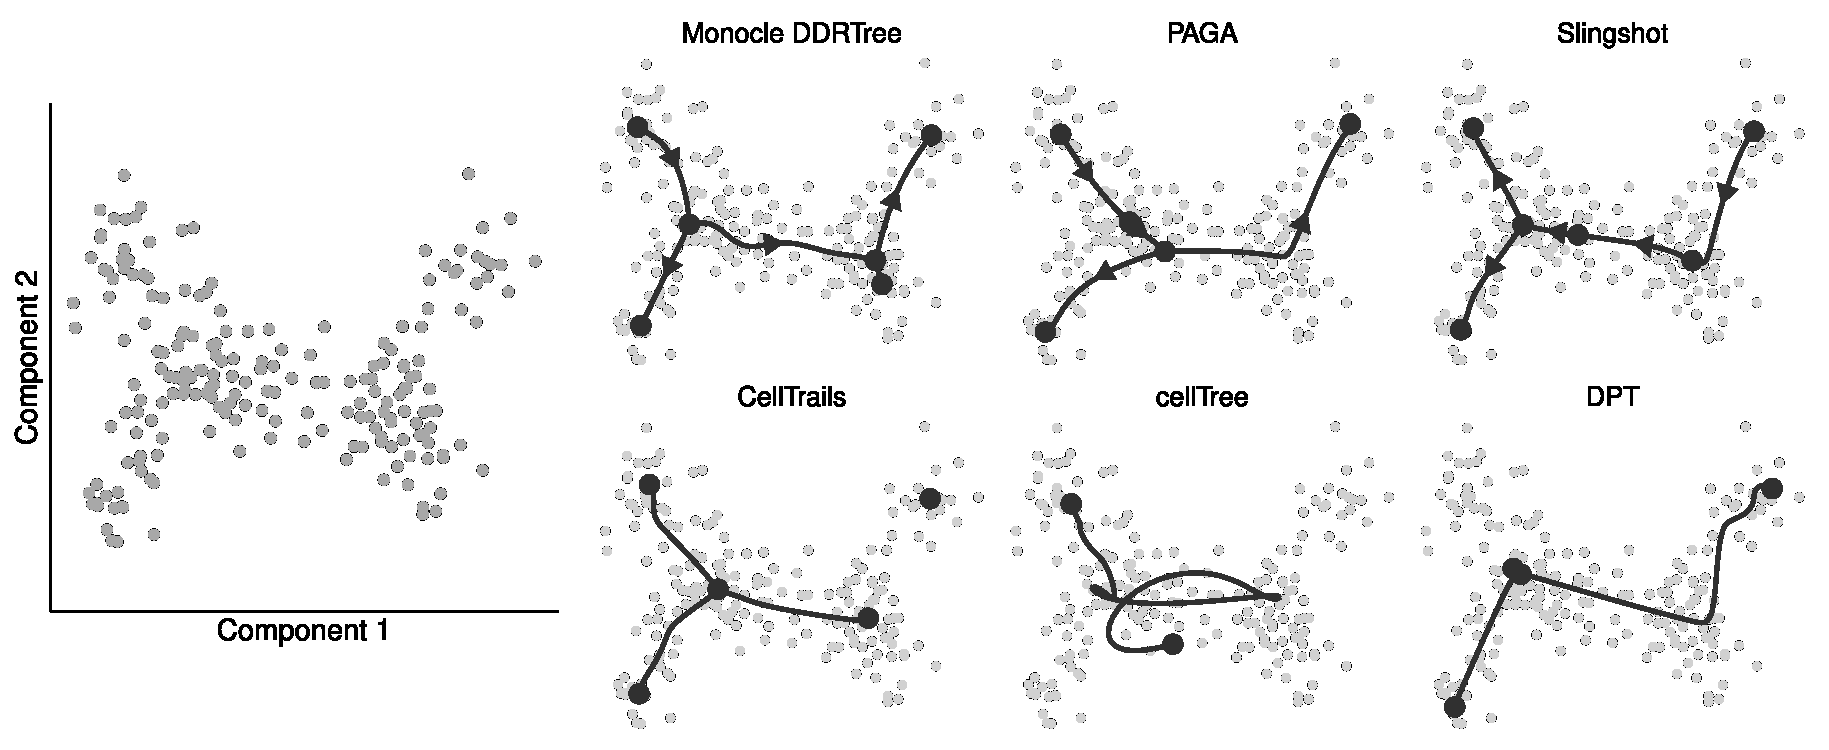
\includegraphics[width=\linewidth]{figures/6_multifurcation/plots_2.pdf}}%
		\only<4->{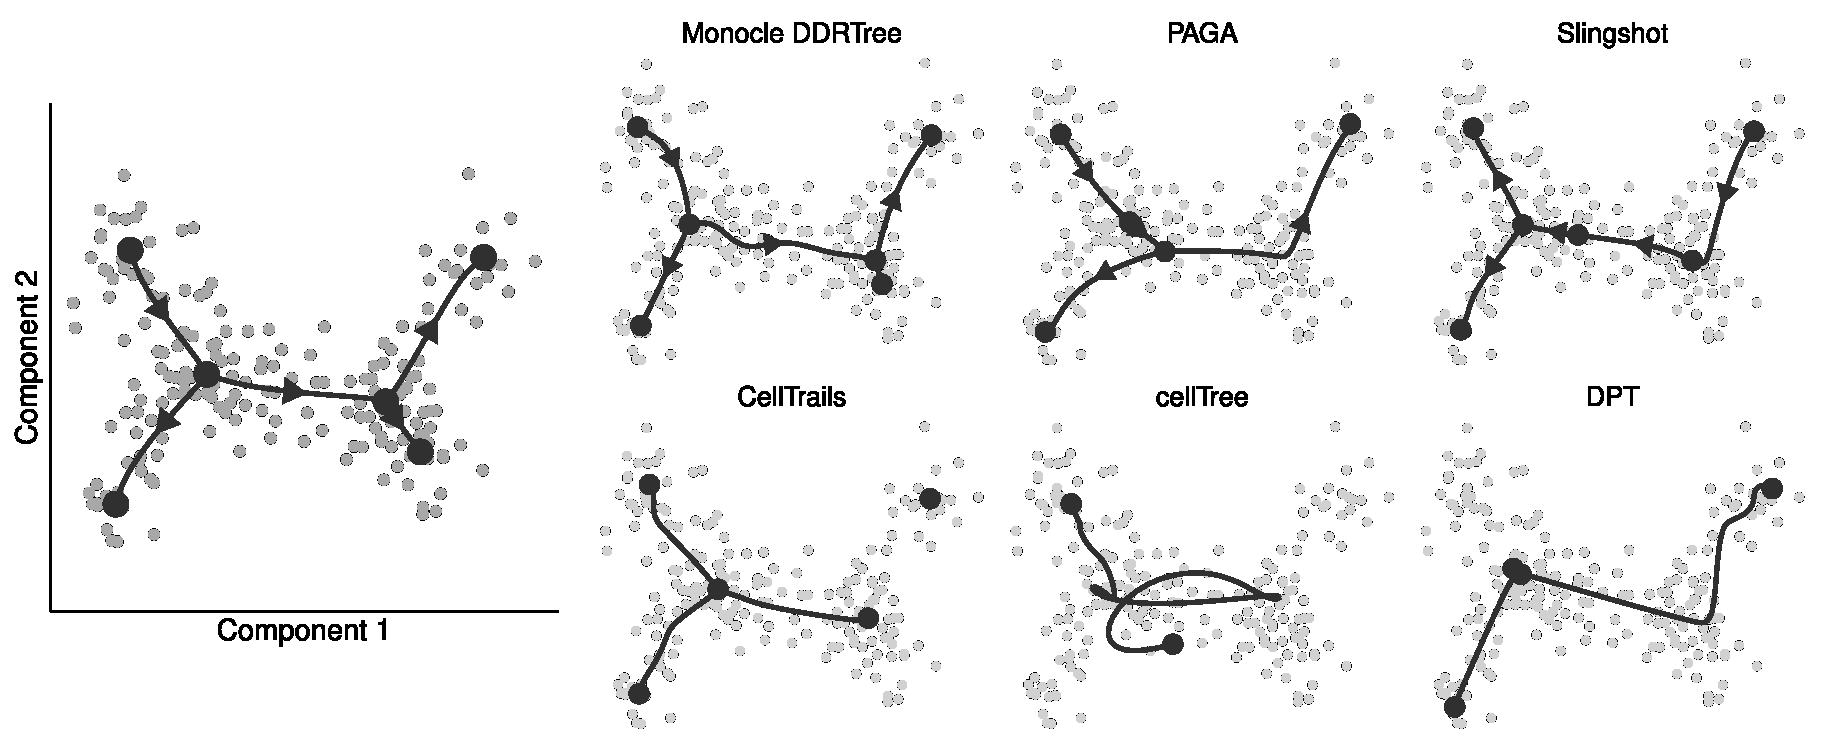
\includegraphics[width=\linewidth]{figures/6_multifurcation/plots_3.pdf}}%
	\end{center}
  \uncover<3->{Trajectory inference; >70 methoden}\\
  \uncover<5->{Nood aan een vergelijking van methoden}
\end{frame}

\begin{frame}
	\frametitle{Simulatie van virtuele cellen}
	\begin{center}
		\movie{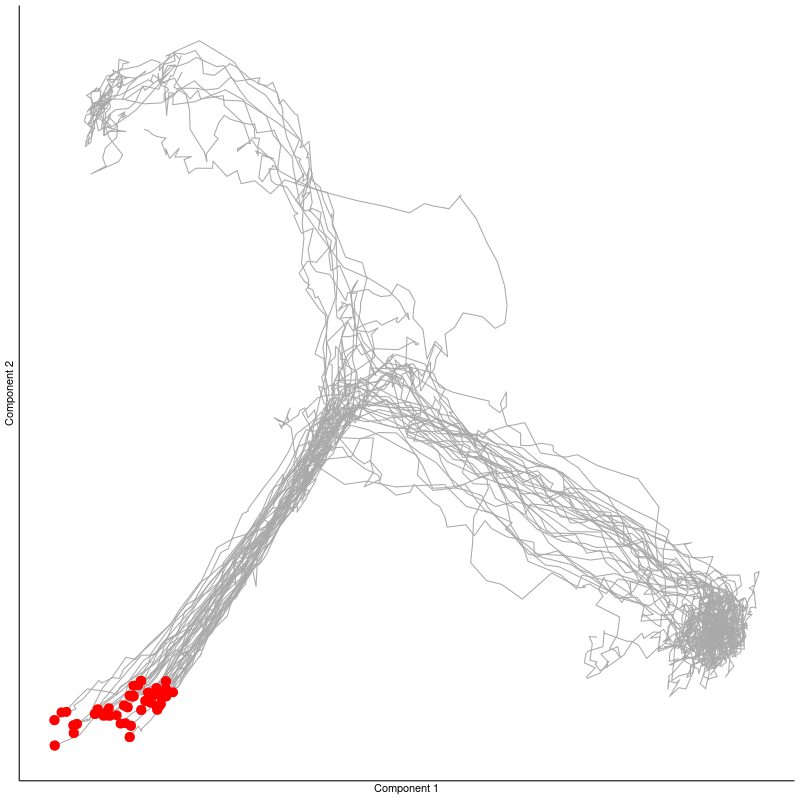
\includegraphics[width=.6\linewidth]{figures/7_dyngen/insilico_init.png}}{figures/7_dyngen/insilico.avi}
	\end{center}
\end{frame}

\begin{frame}
	\frametitle{Simulatie van virtuele cellen}
	\begin{center}
		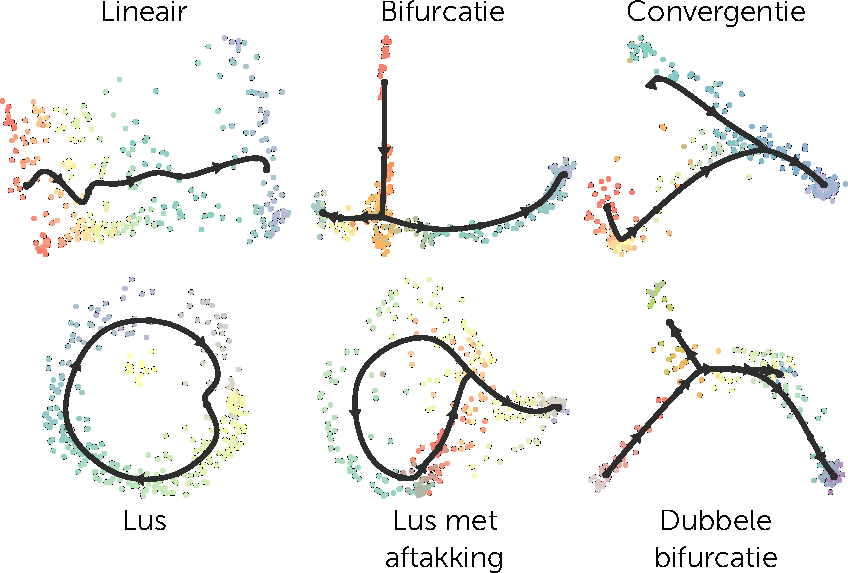
\includegraphics[width=\linewidth]{figures/7_dyngen/example_runs.pdf}
	\end{center}
\end{frame}

\begin{frame}
	\frametitle{Resultaten benchmark}
\end{frame}

\begin{frame}
	\frametitle{Guidelines}
\end{frame}

\begin{frame}
	\frametitle{Conclusies benchmark paper}
\end{frame}

\begin{frame}
	\frametitle{Toekomstvisie}
	\begin{itemize}
		\item Werk Helena rond GNG (toon filmpje)
		\item Trajectory alignment
		\item Combinatie met spatial omics
		\item Human Cell Atlas (vergelijk met de human genome project)
	\end{itemize}
\end{frame}

\end{document}